%necesario para cargar Arial

%:Clase del documento
\documentclass[fontsize=10pt, a4paper, twoside, openany
%, numbers=noenddot % to remove the dot in chapters/sections/figures/
%,svgnames%To use these colors in your LaTeX document, simply include \usepackage[svgnames]{xcolor} in your preamble and then select a color with the \color{} command
%, x11names% xcolor package offers under the option x11names
%,override
,openright]{%article
book}

%-------------------------------------------------

%-------------------------------------------------


\usepackage{subcaption} %  for subfigures environments 
\usepackage[svgnames, x11names,override]{xcolor}
\usepackage[english]{babel}
\definecolor{uccolor}{RGB}{1, 92, 101}
\usepackage{float}
%:Paquete de estilos propuesto
\usepackage{AUXILIARES/estiloTFG}
%:Paquete para incorporar aspectos concretos de la edición  de los apuntes como libro(Portada....)
\usepackage{AUXILIARES/edicionTFG}
%------------------------------------
\usepackage{afterpage}
\usepackage{makeidx}
\makeindex
\usepackage[cp1252]{inputenc}
%----------------------------------------


 \usepackage{graphicx} 
\graphicspath{{./IMAGENES/}{./CAP1/IMAGENES/}{./CAP2/IMAGENES/}}%   Ruta de las imágenes, por capítulos en la carpeta imá‡genes



\usepackage[parfill]{parskip}    % Comienza los párrafos con una línea vacia en vez de con un indentado



\usepackage{pdfpages}  % permite incluir Pá‡ginas de otro documento pdf 
\usepackage{multimedia}% Para incluir videos


%\boldmath  % Para que las f—órmulas resalten

\usepackage{booktabs} % Allows the use of \toprule, \midrule and \bottomrule in tables



%%%%%%%%%%%%%%%%%%%%%%%%%%%%%%%%%%%%%%%%%%%%%%%%%%%%%%%%%%%%

%Para definir el tama–ño del documento, hay que elegir uno de los siguientes y comentar el otro
%Formato Libro
\geometry
{paperheight=300mm,%240mm,%
paperwidth=210mm,%
top=25mm,%
headsep=7.5mm,%
footskip=10mm,%
textheight=250mm,%190mm,%
textwidth=150 mm, %124mm,%
bindingoffset=10mm,%
twoside}


%-----------DEFINIENDO LA ESTRUCTURA DE LA PçGINA-------------------------------------------------%
%%------------------ Margen izquierdo(una pulgada por defecto) y anchura cuerpo -------------------%
%
%\hoffset=0 cm%-0.5cm                        % Margen izquierdo = 2.54cm + \hoffset           %
%
%\textwidth=17cm                                  % Ancho de Pá‡gina(cuerpo)                        %
%%------------------ Control horizontal -----------------------------------------------------------%
%
%\evensidemargin=0cm                              % Distancia margen-cuerpo en Pá‡gina izquierda    %
%
%\marginparwidth=0cm                              % Espacio para notas al margen                   %
%
%\marginparsep=0cm                                % Separaci—ón entre cuerpo y notas al margen      %
%
%\marginparpush=0cm                               % Vertical spacing between sidenotes   %
%
%\oddsidemargin=0.51cm                            % Espacio para encuadernar (derecha e izquierda) %
%%------------------ Margen superior y altura del cuerpo de Pá‡gina --------------------------------%
%
%\voffset= 0 cm%-1.5cm        julio                          % Margen superior = 2.54cm + \voffset            %
%
%\textheight=25.9cm      %24.4cm   julio                 % Altura del cuerpo (zona imprimible) de Pá‡gina  %
%
%%------------------ Control vertical -------------------------------------------------------------%
%
%\topmargin=0cm                                   % Separació—n entre margen superior y cabecera    %
%
%\headheight=0.cm                                % Altura de la cabecera                          %
%
%\headsep=0.6cm                                   % Separaci—n entre cabecera y cuerpo             %
%
%%\footskip=1.5cm                                 % Separaci—n cuerpo-pie Pá‡gina(se incluye Žste)  %
%
%%\parskip=0.2cm                                  % Separaci—ón de pá‡rrafos                         %
%
\renewcommand{\baselinestretch}{1.6}             % Separaci—ón entre líneas              
%
%%%%%%%%%%%%%%%%%%%%%%%%%%%%%%%%%%%%%%%%%%%%%%%%%%%%%%%%%%%%%


%%------------------ Definición del estilo de Capítulo---------------------------------------------%
%\usepackage{lmodern}
%\usepackage{titlesec}
%\usepackage{microtype}
%\titleformat{\chapter}[display]
% {\filcenter\normalfont\bfseries\color{uccolor}}
% {\filleft\hfill%
%\rotatebox[origin=c]{90}{%
%\normalfont\color{uccolor}\Large%
%\textls{\textsc{\chaptertitlename}}%
%}\hspace{10pt}%
%{\setlength\fboxsep{0pt}%
%\colorbox{uccolor}{\parbox[c][3cm][c]{3cm}{%
%\centering\color{white}\fontsize{80}{90}\selectfont\thechapter}%
%}}%
%\\
%\chaptertitlename\\
%}
%{10pt}
%{\titlerule[2.5pt]\vskip3pt\titlerule\vskip4pt\LARGE\sffamily}




%%%%%%%%%%%%%%%%%%%%%%%%%%%%%%%%%%%%%%%%%%%%%%%%%%%%
%\includeonly{} Para introducir solo algunos capitulos

%\usepackage{helvet}
%\renewcommand{\familydefault}{\sfdefault}
%xelatex
%\usepackage{fontspec}
%\setmainfont{Arial}

\usepackage{lipsum}  



\begin{document}


%%%%%%%%%%%   Portada   para article
%:Para crear la portada y la portada interior (pagina titular)
\titulo{ALTEA GEODA}
\subtitulo{Forest Segmentation from Satellite Imagery Using Convolutional Neural Networks for Power Infrastructure Protection in Cantabria} %Se puede usar e	n libro
%\edicion{1ª Edición} %Se puede usar en libro
\autor{Shaokai Chen}
\director{Celestino Guemes Seoane (Tutor empresarial)}
\codirector{Daniel García Díaz}
\edicion{}
\departamento{}
\lugar{Facultad de Ciencias}
\centro{Facultad de Ciencias}
\universidad{Universidad de Cantabria}
\fecha{\today}
\nombregrado{MÁSTER EN CIENCIAS DE DATOS}
\nombretrabajo{University \\ Master's \\ Degree in \elnombregrado }
\isbn{}
\rpintelectual{}



%:Construcción de una cubierta (título a color)
%\cubiertalibro{logo50calidad} 
% Construcción de la portada
\paginatitulo 
\letrafont


%:Todo lo que constituye la primera parte del libro que no es el cuerpo del libro (de apuntes)
%\frontmatter
\pagenumbering{Roman} %Pone la numeración en mayúscula (En español parece que es obligatorio)

%:La dedicatoria, si queremos ponerla


% Poner Resumen
\include{./CAPITULOS/agradecimiento}
\include{./CAPITULOS/resumen}
% Activate the following line by filling in the right side. If for example the name of the root file is Main.tex, write
% "...root = Main.tex" if the chapter file is in the same directory, and "...root = ../Main.tex" if the chapter is in a subdirectory.
 
%!TEX root =  ../plantillaTFG.tex 
%recuerda que si cambias el nombre del fichero... debes cambiarlo aqui
\chapter*{Summary}
Vegetation encroachment on high-voltage power lines poses a critical risk to energy infrastructure, with potential consequences including power outages and wildfire ignition. This project focuses on vegetation control through remote sensing (satellite imagery analysis) in the Cantabria region, with the objective of detecting risk zones where vegetation may potentially come into contact with power lines. To achieve reliable results, four convolutional neural network (CNN) architectures were implemented and evaluated for the task of forest segmentation. Based on a comparative evaluation, DeeplabV3+ was found to outperform the other models in terms of accuracy, F1-score, and AUC. This architecture was therefore selected and applied to generate detailed forest segmentation maps of Cantabria, which were subsequently used to identify and analyze potential vegetation–power line interaction zones.
%\abstractfont 
\setcounter{page}{4}
\printindex


%Índice normal,  completo
%\newpage
\phantomsection
\hypersetup{pageanchor=true,
    linktoc=all,
    linkcolor={uccolor},
    citecolor={uccolor},
    urlcolor={uccolor}  }
%\addcontentsline{toc}{listas}{Indice}
%\pagestyle{especial}
%\setcounter{page}{1}
%{\color{black}
\tableofcontents
%\cleardoublepage


%:Empieza el contenido en si
\mainmatter%, si fuera un libro 

%:Página por defecto
\pagestyle{rdsimolT} %% En realidad es section la que cambia automaticamente el estilo de página
\hypersetup{pageanchor=true,
    linktoc=all,
    linkcolor={blue},
    citecolor={blue},
    urlcolor={blue}  }
%\pagenumbering{arabic}
\setcounter{page}{7}
% Activate the following line by filling in the right side. If for example the name of the root file is Main.tex, write
% "...root = Main.tex" if the chapter file is in the same directory, and "...root = ../Main.tex" if the chapter is in a subdirectory.
 
%!TEX root =  ../plantillaTFG.tex 
%recuerda que si cambias el nombre del fichero... debes cambiarlo aqui
\chapter{Introduction}
%\normalfont
 
\section{Semantic segmentation}
%\lettrine[lines=3]{\color{sepia}E}{}
In recent years, convolutional neural networks (CNNs) have become one of the most widely used machine learning techniques for the researchers in the field of computer vision. Many extensive applications of these models have come up within the rise of different CNN-based architectures, including medical image analysis (detection of diseases from CT or MR images), facial recognition (identify and verify the individuals in the images), object detection (detection of a specific object in the images or videos) and the very trending image fusion and generation using advanced architectures such as diffusion models.\\ 

Some of these applications can be grouped under a field known as semantic segmentation, which focuses on partitioning an image into multiple regions by classifying each pixel into a predefined category. For example, in medical imaging, some segmentation techniques have been used to perform identification of region-of-interest [1], like tumors, organs or other biological structures.\\ 

Another use of CNN model in the segmentation field is the land cover classification (Figure 1.1), which involves analyzing satellite or aerial images and labeling each pixel with classes such as water, forests, urban areas, agricultural lands, etc. These models are usually used for environmental monitoring to help track changes in natural habitats, deforestation rates, or water resource distribution over time [2].\\
\begin{figure}[h]
 \centering
 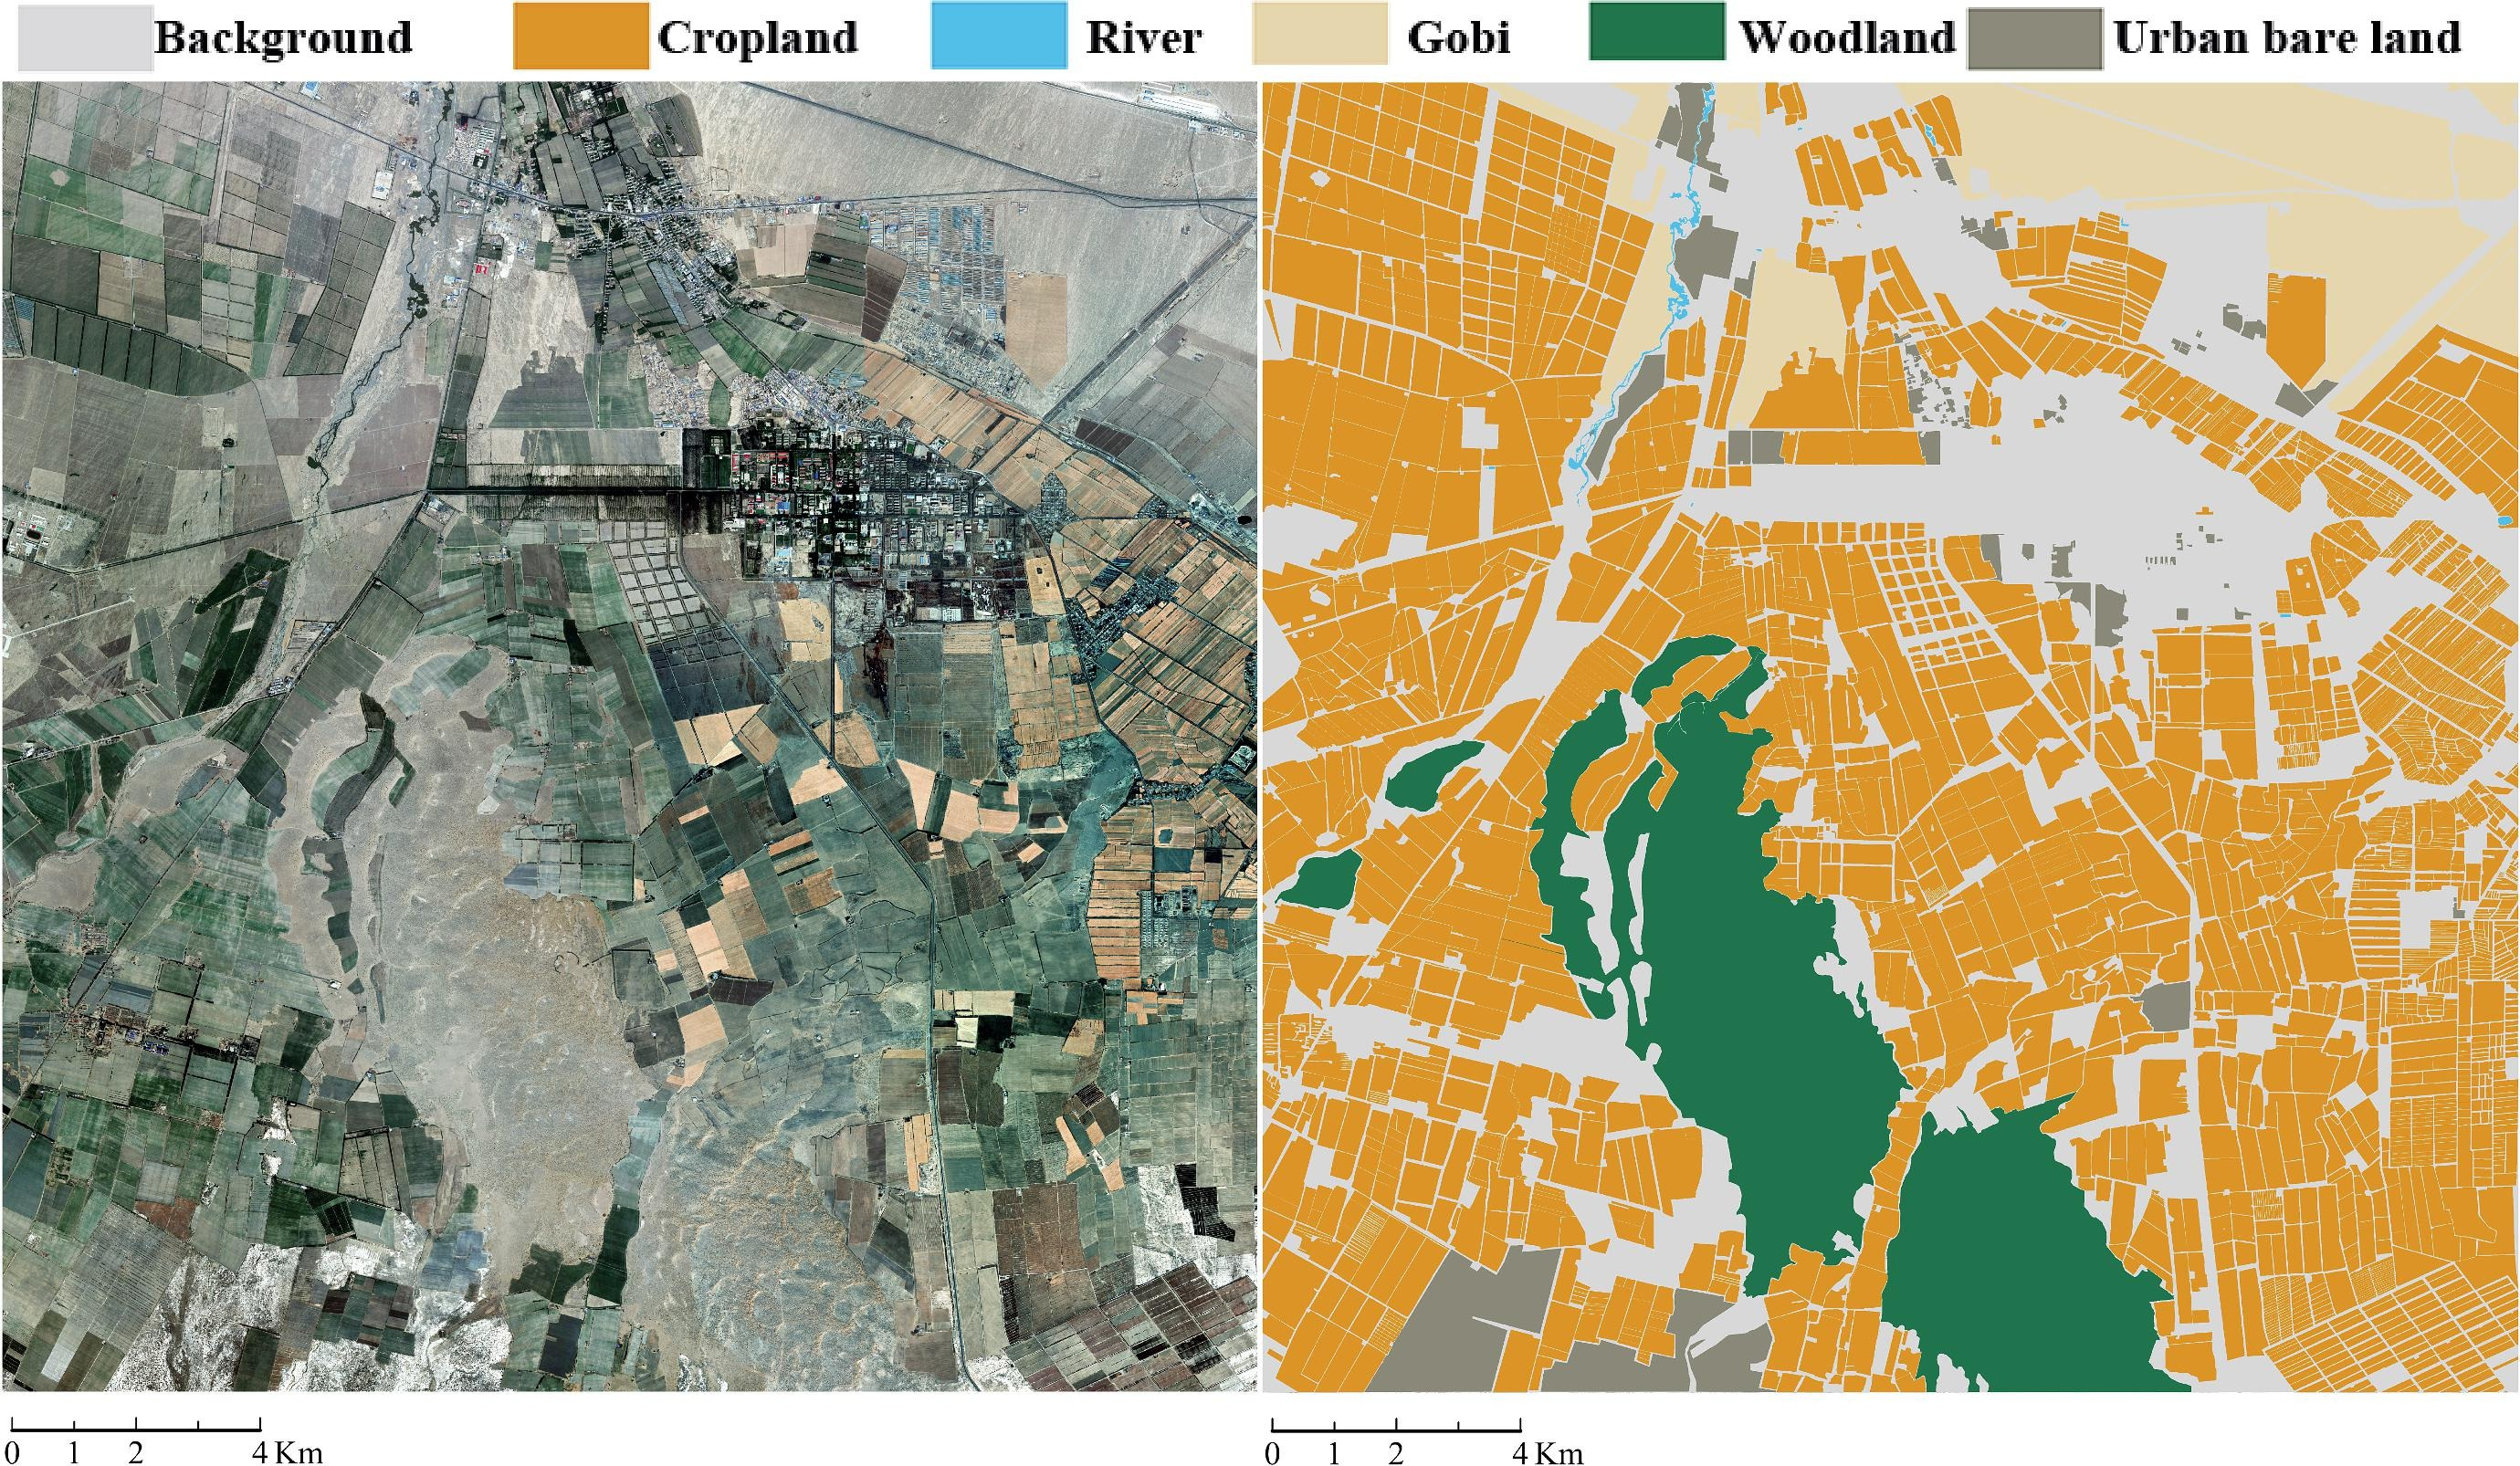
\includegraphics[scale=1.05]{IMAGENES/IMG1-Introduction.jpg}
 \captionsetup{font=large}
 \caption {Example of land cover segmentation. The left side shows the satellite image; the right side shows its ground truth mask. The image is segmented into six categories: Background, Cropland, River, Gobi, Woodland, and Urban bare land (image extracted from [1])}
\end{figure}


In this project, we focus on one specific subsection of land cover analysis: forest segmentation. The aim of the project is to monitor the spatial distribution and extent of forests in Cantabria, in order to detect changes and identify potential risks, such as the proximity of tree canopies to high-voltage power lines, which can result in severe incidents, including electrical short circuits, power outages, and even the ignition of wildfires. By using advanced image analysis and segmentation techniques, we will be able to map prediction mask on satellite imagery, assess their growth patterns, and identify risk zones where vegetation management is necessary. 

\newpage
\section{Motivation}
The project forms part of the internship at Alten-Worldgrid, a company that specializes in providing IT solutions to clients in the energy sector. For some of the clients, particularly those working with the operation and maintenance of electricity transmission networks, the potential contact between the tree canopies and high-voltage power lines has always been a major risk. There have been many reports [12,13] related to wildfires caused by the ignition of vegetation around utility poles. Such incidents may be triggered by overgrown tree canopies that come into contact with power lines or by extreme weather conditions that cause nearby trees to fall onto the lines.
\\


To prevent these kinds of problems, one commonly used approach is to send teams periodically to inspect and carry out vegetation maintenance operations to the areas near the power lines, this typically involves sending personnel to either prune overgrown branches or, when necessary, cutting down trees entirely. However, this task often requires a lot of human resources, financial investments, and it presents 2 main inconveniences:\\

\begin{itemize}
\item \textbf{Where?} Since the entire power line network is large and is widely distributed across country, it is difficult to determine the exact locations that need to perform pruning.
\item \textbf{When?} The is also a lack of information about the optimal timing for pruning, and sending teams periodically is not usually an efficient approach and might be costly.
\end{itemize}



\textbf{Proposed approach}: 

To address these challenges, we propose the use of machine learning techniques to identify forested areas and detect high-risk zones. In the other words, train a CNN-based model (or a suite of models) to perform semantic segmentation on satellite imagery. By combining the model outputs with geospatial data on power lines networks, it is possible to highlight the intersection areas and enable the targeted maintenance. 





\chapter{Theoretical Fundamentals}
\section{Introduction to CNNs}

One of the most important elements in CNN models is their hierarchical feature extraction ability. In brief, instead of feeding all raw pixel values directly into a fully connected neural network (FCN), CNNs use convolution operations (also known as the filters) to progressively capture local patterns. The early layers of a CNN learn low-level features like edges, corners, and simple textures. As the network goes deeper, these features can be combined to form higher-level abstractions like eyes, wheels or other shapes, allowing the model to understand more complex structures in the image, in other words, the feature representation gets better in the deeper layers. \\


This feature extraction is achieved by sliding a fixed size filter (usually 3x3) over the input feature map (or input image, in the case of the first layer), multiplying each filter value by the corresponding feature value, and then summing all the results to generate an output value, after going through an activation function, this output becomes the element of the feature map for the next layer. \\
\begin{figure}[H]
 \centering
 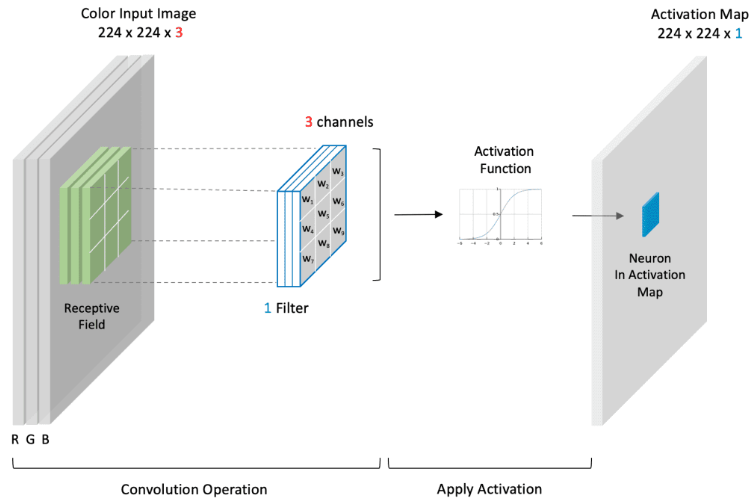
\includegraphics[scale=0.53]{IMAGENES/IMG2-Convolutional_operation.png}
 \captionsetup{font=large}
 \caption {Scheme illustrating the process of a convolutional operation: a 3 x 3 × 3 filter slides over a 224 × 224 × 3 input image, the outputs generated will become the input feature map for the deeper layer. (Image extracted from [2]) }
\end{figure}


In the model architecture, these layers responsible for feature extraction are typically grouped into a module or block called the “backbone”, and it includes all convolution, activation and pooling layers. Once feature extraction is complete, a task-specific block, called the “head”, is applied to produce the final output. For example, for classification tasks, it is common to apply an FCN with a SoftMax activation as the head, as for the classification usually requires a fixed-length output vector with as many elements as classes. Whereas for segmentation tasks, a convolutional layer with a sigmoid activation is usually used, in order to produce a pixel-wise probability mask (2 classes). For multiclass segmentation, a Softmax activation is used across the channel dimension to produce a multi-channel probability map, with one channel per class.\\


Note that “backbone” and “head” are not considered to be universal technical terms, but they are used in some articles and some machine learning frameworks such as PyTorch and Tensorflow to describe the process of transfer learning[3], which is a commonly used technique in model training. In transfer learning, it is common to use a backbone that has been previously trained on a large dataset, it will serve as a general-purpose feature extractor. Then a task-specific head will be added, and the final composite model can be retrained on the target dataset through fine-tuning for the specific task.\\

\section{Model architectures}
One of our objectives in this project is to identify the model architecture that best fits our segmentation task. Therefore, we have selected several CNN-based models and evaluated their performance on our target dataset, which will be discussed in the Model Training section.\\

Next, we will describe shortly each of the model architectures that were evaluated: 
\subsection{2.2.1 U-Net}
\begin{figure}[H]
 \centering
 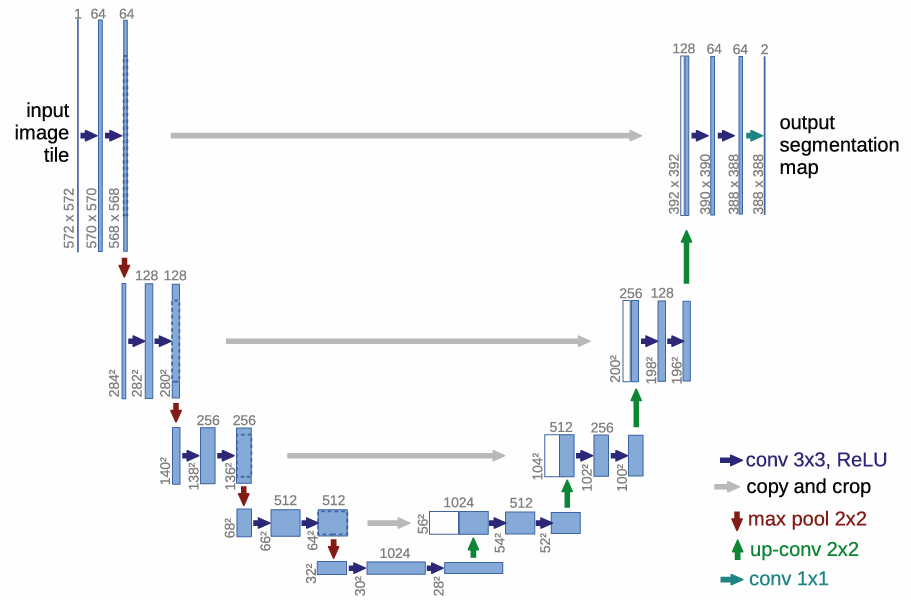
\includegraphics[scale=0.6]{IMAGENES/IMG3-UNet.PNG}
 \captionsetup{font=large}
 \caption {UNet architecture. (Image extracted from [4]) }
\end{figure}

The U-Net is a widely used architecture for segmentation tasks, it was first introduced in (O. Ronneberger, P. Fischer, and T. Brox: "U-net: Convolutional networks for biomedical image segmentation") [4], as the title suggests, the architecture was originally designed for medical image segmentation, in this project we decided to test its performance on our task because, on the one hand, it is simple to implement so it can be a good starting point for experimentation. And on the other hand, we consider that the biostructure identification task is similar to our forest segmentation task since both involve detecting complex patterns and irregular structures. \\


One of the key characteristics of U-Net is its U-shape structure, it consists of a contracting path (encoder) and an expansive path (decoder). The contracting path is generally formed by a series of convolution-pooling blocks (encoder blocks). Each block contains several convolution layers followed by ReLU activations and a max pooling layer. In the contraction process, the max pooling layer progressively reduces the size of the input tensors (input feature maps), forcing the model to learn global context at the cost of losing fine-grained details (which will later be recovered using skip connections). This can also be seen as increasing the receptive field of the neurons (area that each neuron can “see”)[9], since the size of tensors is progressively reducing, a 3x3 filter can cover more information each time . \\


The expansive path is formed by up-convolution blocks (decoder blocks). These blocks enlarge the input tensors back to a higher resolution, and they are linked with their corresponding encoder block through skip connections. In this way, high-resolution tensors from the contracting path will be passed to the expansive path and concatenated with the decoder tensors, helping the model to alleviate the information loss problem and generate a more precise output. \\

\subsection{2.2.2 U-Net++}
\begin{figure}[H]
 \centering
 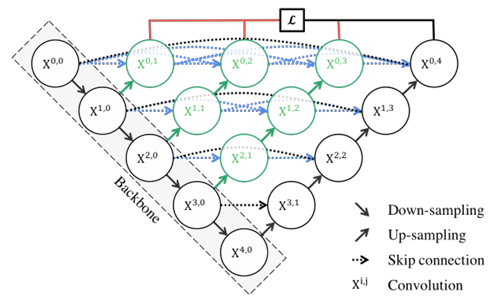
\includegraphics[scale=0.9]{IMAGENES/IMG4-UNetPP.PNG}
 \captionsetup{font=large}
 \caption {UNet++ architecture. (Image extracted from [4]) }
\end{figure}

The original U-Net architecture has been extensively used in many biomedical image segmentation studies due to its remarkable performance, thus, many variants have been designed to further increase segmentation accuracy and robustness.\\


U-Net++ is one of its variants [5], it has a more complex structure than the original U-Net. The main distinction between them resides in the introduction of an additional convolution module (marked as green in the Figure 2.3) that acts as bridges connecting the encoder and decoder. Unlike in the conventional U-Net, where the feature maps of the encoder are passed directly to the decoder, in U-Net++ these maps go through a dense convolution module before being passed to it. The main idea is to bridge the semantic gap between the feature maps of the encoder and decoder prior to fusion, which might make the optimization problem easier [5].\\

\subsection{2.2.3 Attention U-Net}
\begin{figure}[H]
 \centering
 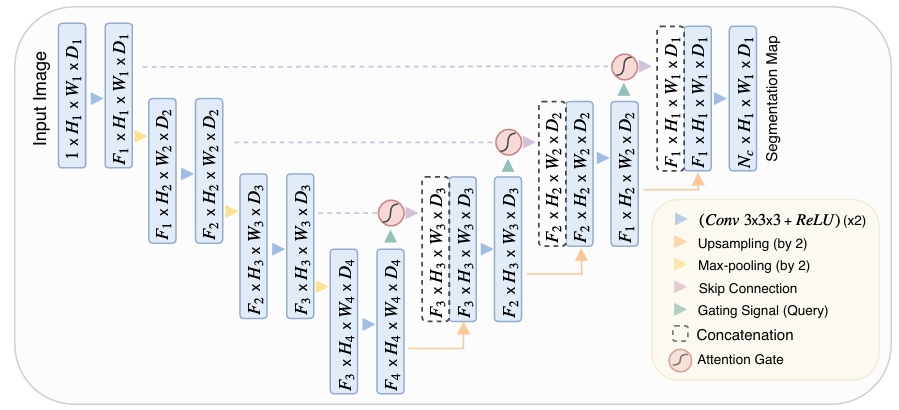
\includegraphics[scale=0.6]{IMAGENES/IMG5-AUNet.PNG}
 \captionsetup{font=large}
 \caption {Attention UNet++ architecture. (Image extracted from [6]) }
\end{figure}

Attention U-Net is another variant of the U-Net architecture that introduces attention mechanisms to improve feature extraction [6]. In this variant, an attention gate is integrated into the skip connections. The feature maps from each encoder block pass through the attention gate before being concatenated with the corresponding decoder tensor.\\

The purpose of the attention gate is to help the model to focus more on target structures of varying shapes and sizes. According to the original ariticle [6], models trained with attention gates are able to suppress irrelevant regions in the input image while emphasizing salient features that are important for the task.\\

The architecture of the attention gate is shown in the following figure: 

\begin{figure}[H]
 \centering
 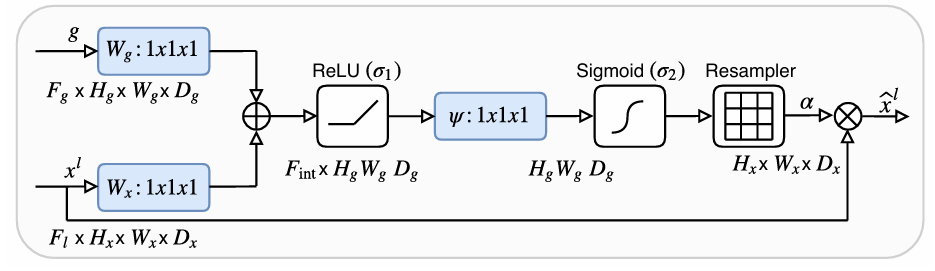
\includegraphics[scale=0.6]{IMAGENES/IMG6-AttentionGate.PNG}
 \captionsetup{font=large}
 \caption {Attention gate architecture. (Image extracted from [6]) }
\end{figure}

The gate mechanism has been well explained in (R. Vinod, “A detailed explanation of the attention u-net.”) [7]. To summarize, the gate receives 2 inputs: the tensor x from the current-level layer, and the tensor g (also known as the signal) from the next-level layer. The tensor g has a smaller dimension but carries better feature representations since it comes from a deeper layer.\\

Both tensors go through a 1x1 convolution (tensor x undergoes an additional max pooling operation to match the spatial dimensions of g). The 2 processed tensors are then summed elementwise, the resulting tensor will have larger values in regions where the weights are aligned, and smaller values where they are not. Then, the tensor will go through a series of convolution-activation blocks and a resampling operation to restore it to the original dimensions of x, obtaining in this way a coefficient tensor called alfa.\\ 

The alfa contains information about the regions-of-interest (regions where the weights are higher) and is used to scale x via elementwise multiplication. This gated tensor is then passed to the decoder blocks through skip connections.\\

\subsection{2.2.4 DeeplabV3+}
\subsection{- Problems in the U-Nets }
The previous architectures are all variants of U-Net, and thus they all share a common limitation: the spatial resolution progressively decreases as the network goes deeper. As explained in the U-Net section, this aims to increase the receptive field of neurons, so that the network can capture global contextual information. This action is usually beneficial for the classification tasks since they require a global understanding of the image. However, it might be harmful for the segmentation tasks, which depend heavily on the spatial information. In other words, as the network goes deeper, it gains more information of “what object is in the image?” but gradually loses information about “where the object is located?”.\\

The key point to alleviate this problem is to increase the receptive field while preserving the spatial resolution. One way to achieve this is by using larger filter sizes (for example, 7x7 instead of 3x3). Since a larger filter can cover a wider area of the input, it allows the network to capture global context without requiring additional spatial reduction. Nevertheless, using a larger filter would also increase the number of parameters and, consequently, the computational complexity. As a solution, the dilated convolutions (also known as atrous convolutions) have been proposed. [10]\\

\subsection{- Dilated convolutions }
\begin{figure}[H]
 \centering
 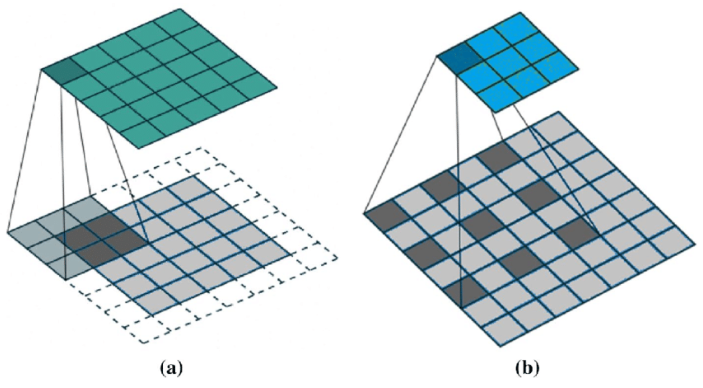
\includegraphics[scale=0.6]{IMAGENES/IMG7.PNG}
 \captionsetup{font=large}
 \caption {a) Traditional convolution. b) Dilated convolution (Atrous convolution) with dilation rate = 2. (Image extracted from [7]) }
\end{figure}

The architecture itself is simple to understand, it can be visualized as a standard convolutional filter with “holes”, created by stretching the original filter so that it can capture a larger portion of the image at once. The number of filter parameters remains unchanged (3x3 parameters), but the filter itself is dilated by inserting gaps between its values, and the pixels corresponding to these gaps are skipped and not taken into account during the elementwise multiplication.\\

The size of the gaps is controlled by a hyperparameter r (also known as the dilation rate). When r=1, the filter reduces to a normal convolutional filter, with no gapes between its elements, and as r increases, the receptive field grows exponentially without increasing the number of parameters. 

\subsection{- ASPP }
\begin{figure}[H]
 \centering
 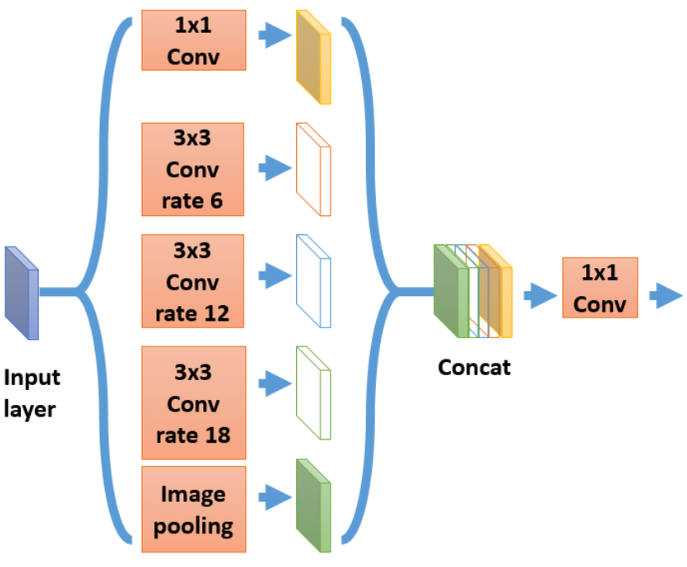
\includegraphics[scale=0.6]{IMAGENES/IMG9-ASPP.PNG}
 \captionsetup{font=large}
 \caption {ASPP module, the module is formed by multiple dilated convolution layers in parallel (Image extracted from [9]) }
\end{figure}
Based on the dilated convolution technique, the Atrous Spatial Pyramid Pooling (ASPP) module has been developed to address another challenge that the U-Nets are facing [14]: An object can appear at different scales in the images. The difficulty of detecting varying sizes objects can usually be alleviated by providing rescaled versions of the same input image to the network. Inspired by this idea, ASPP employs multiple parallel dilated convolutional layers with different dilation rates. Each dilated convolutional layer in ASPP samples the input at a specific resolution to capture the object at that scale, and the outputs of these layers are then concatenated together to produce the final result. 

\subsection{- DeepLabv3+ arquitecture}

One of the most successful models built on the previous techniques is DeepLabV3+ [14], it is the latest successor in the DeepLab series, designed by google researchers for a variety of semantic segmentation tasks. DeepLabV3+ uses a ResNet model as the backbone along with dilated convolutions and ASPP module. The model architecture is shown in the figure below: 

\begin{figure}[H]
 \centering
 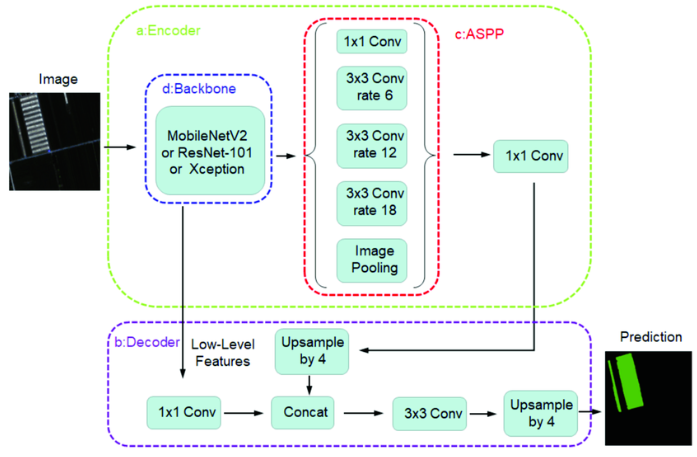
\includegraphics[scale=0.8]{IMAGENES/IMG8-deeplab.PNG}
 \captionsetup{font=large}
 \caption {DeepLabV3+ architecture scheme. The scheme shows an encoder block (a) that contains a ResNet module (d), which acts as backbone for lower-level feature extraction, a ASPP module (c), for multi-scale context extraction. And a decoder block (b), which concatenates the resulting feature maps and up sample them to the original size for final prediction. (Image extracted from [8]) }
\end{figure}

It is important to note that the selection of the backbone is very flexible, ResNet is not a fixed option, for example, it can use a ResNet pretrained on the ImageNet dataset or a MobileNet pretrained on the CoCo dataset [16, 17].  
% Activate the following line by filling in the right side. If for example the name of the root file is Main.tex, write
% "...root = Main.tex" if the chapter file is in the same directory, and "...root = ../Main.tex" if the chapter is in a subdirectory.
 
%!TEX root =  ../plantillaTFG.tex 
%recuerda que si cambias el nombre del fichero... debes cambiarlo aqui
\chapter{Data Preparation}
The main objective of our project is to identify risk zones where potential contact between power lines and vegetation could occur in the region of Cantabria. Thus, satellite imagery data related to vegetation (or more broadly, landcover) is required, along with corresponding masks that outline vegetation areas for model training (preferably specific to Cantabria, if available). In addition to vegetation data, geospatial data on the location of power lines is also needed for analyzing intersection zones. 
\newpage
\section{Copernicus data}
\begin{figure}[H]
 \centering
 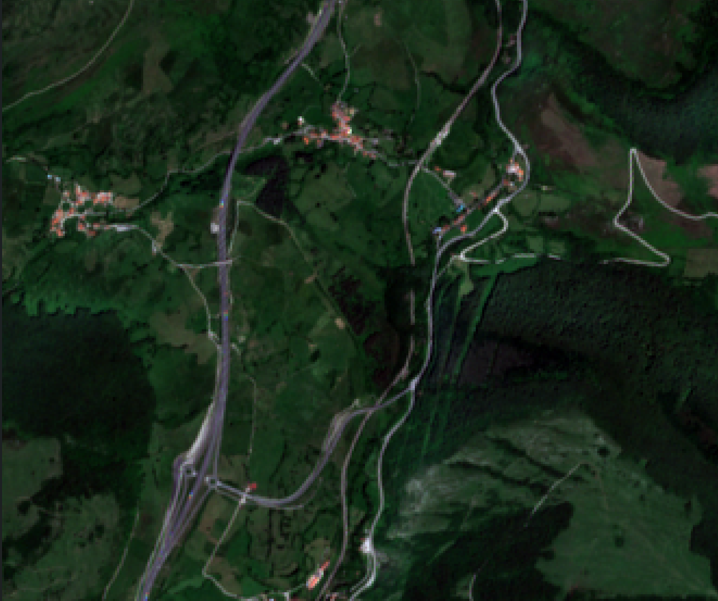
\includegraphics[scale=0.8]{IMAGENES/IMG10-sentinel2.png}
 \captionsetup{font=large}
 \caption {Sentinel 2A imagery, with only RGB channels.}
\end{figure}

For the vegetation dataset, our initial approach was to create a custom dataset. We began by exploring open-access imagery from Sentinel-2 mission. To load and visualize this data, we utilized the Copernicus API with an open-source GIS application called QGIS. The imagery obtained is composed of multiple spectrums in different
spatial resolutions (for example, in visible bands, the resolution is 10 m/pixel), these bands could be used to determine some important indices, such as the Normalized Difference Vegetation Index (NDVI), which is useful for identifying vegetation. However, during the data processing phase, we have encountered 2 problems:\\

\begin{itemize}
    \item \textbf{Complexity in manaing spectrums}: As previously mentioned, the images are composed of multiple spectrums (not just the standard RGB channels), and this presents a problem for model training, because we need to decide whether to include all available spectral bands (Sentinel-2 satellite images include a total of 13 spectral bands) or restrict the input to only the RGB channels. This decision must be made at the beginning, as once a model is trained, its architecture and weights are fixed. Consequently, the model can only perform inference on images with the same number and type of channels used during training. In other words, if the model was trained on all 13 spectral bands, it cannot perform inference on input image that has only RGB bands.\\ 
    \item \textbf{Manual annotation}: These data lack corresponding segmentation masks, meaning that any further processing would require creating them from scratch through manual annotation, which is highly time-consuming and labor-intensive.
    


\end{itemize}
Given the limited timeframe for project implementation, we considered that relying on the initially planned data sources was not feasible. Consequently, an alternative approach was explored, focusing on more suitable sources of satellite imagery that already included pre-annotated masks.
\section{Jordan Forest Dataset (Training set):}
\begin{figure}[H]
\centering
\begin{subfigure}{0.49\textwidth}
\centering
\includegraphics[width = \textwidth]{IMAGENES/IMG11-IMG.jpg}
\caption{Jordan Forest Dataset (Image)}
\label{fig:left}
\end{subfigure}
\begin{subfigure}{0.49\textwidth}
\centering

\includegraphics[width = \textwidth]{IMAGENES/IMG11-MASK.png}
\caption{Jordan Forest Dataset  (Mask)}
\label{fig:right}
\end{subfigure}
\caption{Jordan Forest Dataset (Images extracted from[21])}
\label{fig:combined}
\end{figure}


\textbf{Description}: 
\\
The Jordan Forests Dataset was obtained from a data science community called Kaggle [18]. It contains a collection of 4,576 cloud-free Landsat-8 satellite images, each with a spatial dimension of 2160 x 3840 pixels (30 m/pixel). Despite the images have a lower resolution comparing with those of Sentinel-2 (10 m/pixel for visible bands), the dataset includes both the original RGB satellite images and the corresponding ground-truth forest masks, therefore no manual annotation is required. The imagery spans a ten-year period from 2010 to 2020, covering five major forested regions in Jordan.\\ 

\textbf{Curation}: 
\\
In the ground-truth masks, the forest regions are highlighted in green, while the remaining non-forest areas are considered as background and marked white (these masks are provided in RGB format rather than binary). As part of the preprocessing pipeline, we have converted the masks into binary format, assigning a value of 1 to forested pixels and 0 to the background (non-forest areas).\\

\section{Loveda dataset (Training set):}
 \begin{figure}[H]
\centering
\begin{subfigure}{0.49\textwidth}
\centering
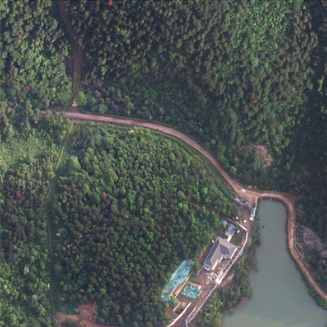
\includegraphics[width = \textwidth]{IMAGENES/IMG12-lov-IMG.PNG}
\caption{Loveda dataset (Image)}
\label{fig:left}
\end{subfigure}
\begin{subfigure}{0.49\textwidth}
\centering

\includegraphics[width = \textwidth]{IMAGENES/IMG12-lov-MASK.PNG}
\caption{Loveda dataset (Mask)}
\label{fig:right}
\end{subfigure}
\caption{Loveda dataset (Images extracted from[18])}
\label{fig:combined}
\end{figure}

\textbf{Description}: 
\\
The LoveDA Dataset was originally designed to support research in both landcover semantic segmentation and unsupervised domain adaptation [20, 21], it is considered to be a benchmark dataset for evaluating the performance of segmentation models in remote sensing tasks. The dataset contains 5987 high spatial resolution (0.3 m/pixel) remote sensing images, each with a spatial dimension of 1024 x 1024 pixels. These images are collected from a diverse set of urban and rural regions across China, and their corresponding masks with landcover labels are also provided in the repository.\\

\textbf{Curation}: 
\\
The masks contain multiple category labels: no data region (0), background (1), building (2), road (3), water (4), barren (5), forest (6), and agriculture (7). For our forest segmentation task, we are only interested in the forested areas. Therefore, the dataset has been filtered to retain only those images where the forest cover exceeds 40\%, resulting in a total of 337 images. Subsequently, the masks were converted into a binary format, with pixels labeled as 1 representing forested areas and pixels labeled as 0 representing non-forested areas. \\



\section{Cantabria dataset (Target set): }
\begin{figure}[H]
 \centering
 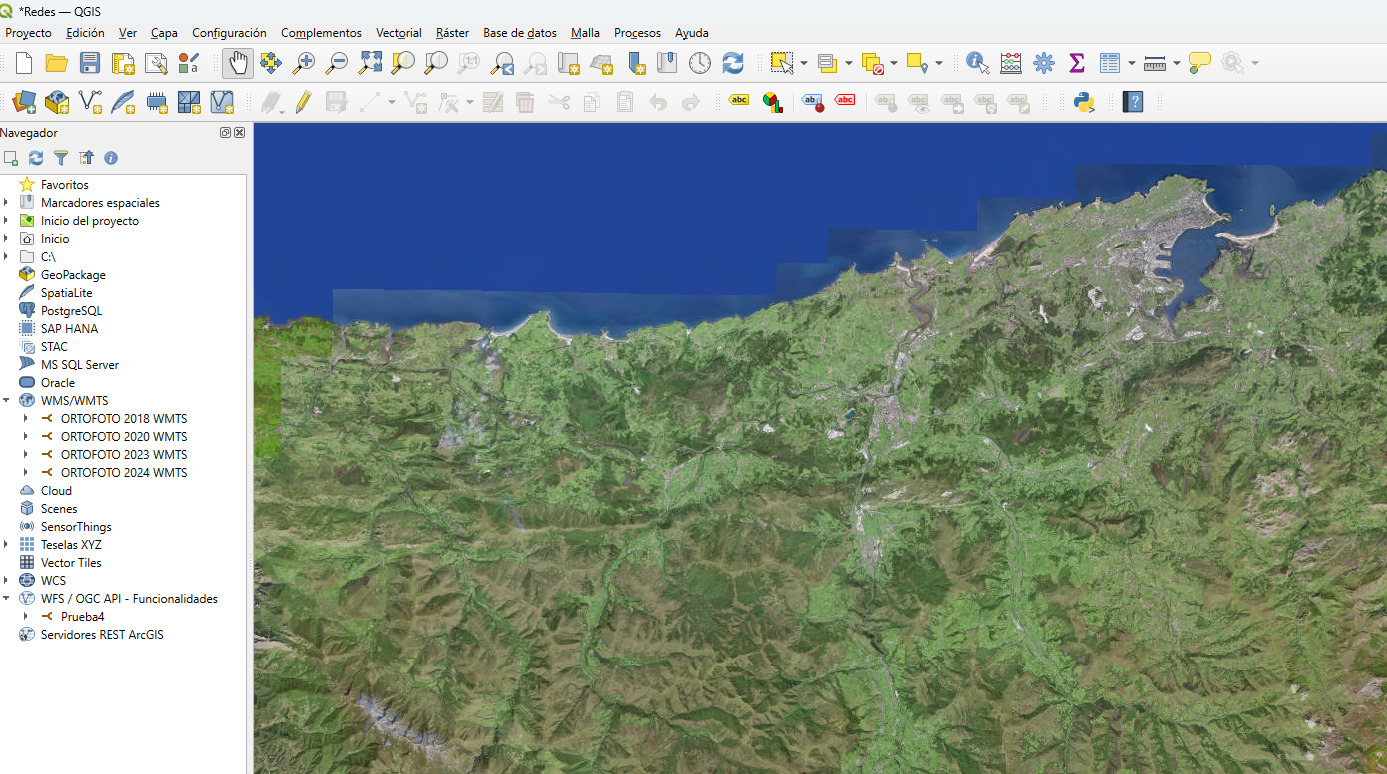
\includegraphics[scale=0.45]{IMAGENES/IMG14-WMTS.png}
 \captionsetup{font=large}
 \caption {Map canvas loaded in QGIS using WMTS.}
\end{figure}

\textbf{Description}: 
\\

Since the study area is Cantabria, satellite imagery of Cantabria is required to perform inference and evaluate the model performance. Fortunately, the government of Cantabria has published high-resolution orthophotos (0.2 m/pixel) covering the region for multiple years, which can be accessed using WMTS (Web Map Tile Service).\\

\textbf{Curation}: 
\\
In order to creat the target dataset for inference, the most recent orthophoto (Figure 3.4) has been loaded into QGIS via WMTS. QGIS displays the orthophotos as pre-rendered image tiles, which are requested from the WMTS server and seamlessly assembled in the map canvas.\\
\begin{figure}[H]
 \centering
 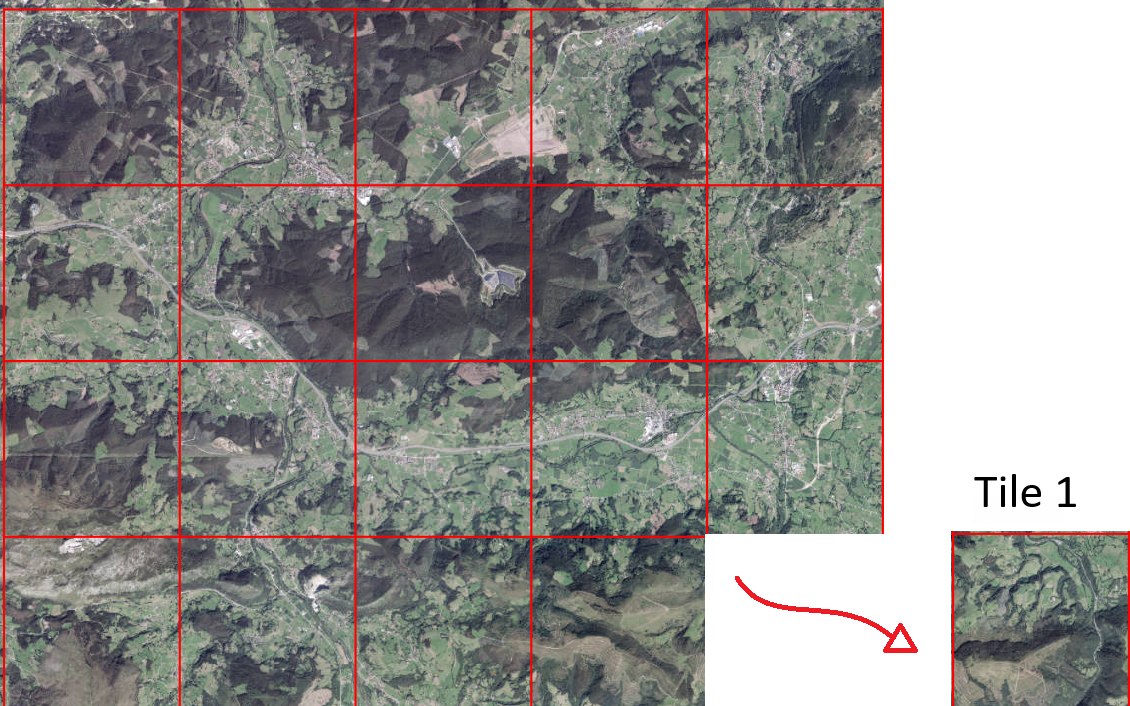
\includegraphics[scale=0.5]{IMAGENES/IMG13-Cantabria.png}
 \captionsetup{font=large}
 \caption {A custom grid with a cell size of 3000mx3000m has been applied to the study area, then, the tiles were exported in PNG format.}
\end{figure}
Once the orthophotos have been loaded, a large region with high vegetation coverage was selected, and a custom grid with a cell size of 3000m x 3000m was applied to the region, dividing it into multiple tiles (Figure 3.5). These tiles were then exported in PNG format along with their corresponding georeferencing information, 
stored in an accompanying pgw files. This process resulted in 70 tiles, each with a spatial dimension of 15000 x 15000 pixels (0.2 m/pixel resolution). The reason to export such large images is to alleviate a problem we encountered during the inference process, which will be explained in the Results section.\\ 

\section{Datasets summary}
The following table summarize the datasets used during the model training:
\begin{table}[H]
\begin{tabular}{|l|l|l|l|l|}
\hline
\multicolumn{1}{|c|}{\textbf{Dataset}} & \multicolumn{1}{c|}{\textbf{Usage}} & \multicolumn{1}{c|}{\textbf{Dimensions}} & \multicolumn{1}{c|}{\textbf{Resolution}} & \multicolumn{1}{c|}{\textbf{Num. of images}} \\ \hline
Jordan Forest                          & Training set                        & 2160 x 3840 pixels                       & 30 m/pixel                               & 4576                                               \\ \hline
LoveDA                                 & Training set                        & 1024 x 1024 pixels                       & 0.3 m/pixel                              & 303                                                \\ \hline
LoveDA                                 & Validation set (Grid search)        & 1024 x 1024 pixels                       & 0.3 m/pixel                              & 34                                                 \\ \hline
Cantabria                              & Target set                          & 15000 x 15000 pixels                     & 0.2 m/pixel                              & 70                                                 \\ \hline
Cantabria\_subset                      & Testing set                         & 1024 x 1024 pixels                       & 0.2 m/pixel                              & 30                                                 \\ \hline
\end{tabular}
\caption{Description of the datasets.}
\label{tab:my-table}
\end{table}

% \begin{figure}[H]
%  \centering
%  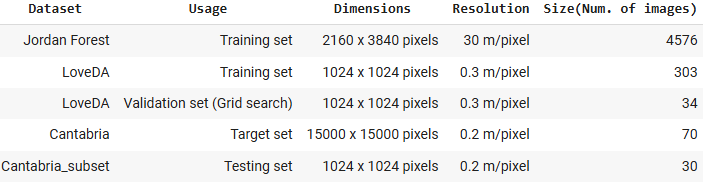
\includegraphics[scale=0.8]{IMAGENES/Dataset_table.png}
%  \captionsetup{font=large}
%  \caption {Description of the datasets.}
% \end{figure}
Both the Jordan Forest and LoveDA datasets were used for model training. The LoveDA dataset was divided into two subsets: one for training and another for validation. The validation set was utilized to perform a grid search in order to determine the optimal hyperparameters for each architecture. Additionally, a supplementary Cantabria subset was created to evaluate model performance on Cantabria images. This subset consists of 30 manually annotated images and served as the testing set.

\section{Power line data: }
\begin{figure}[H]
 \centering
 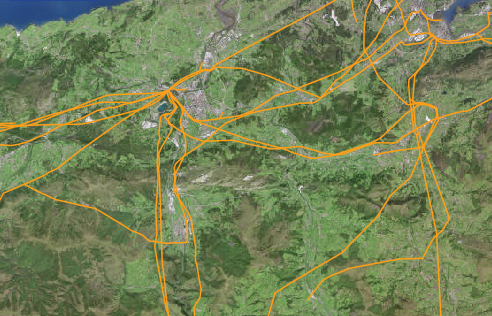
\includegraphics[scale=1.6]{IMAGENES/IMG15-Lines.png}
 \captionsetup{font=large}
 \caption {Power line data.}
\end{figure}

\textbf{Description}: 
\\
The high-voltage power line data are openly accessible through the IDEE websites (Infraestructura de Datos Espaciales de España)[22]. These data form part of a multipurpose geographic dataset called BTN100 (Base Topográfica Nacional 1:100.000). The dataset includes numerous geographic objects represented at the specified scale using simple geometries (points, lines, and polygons), each enriched with thematic information stored in attribute fields. These objects cover diverse topics, such as administrative unity, transport, water deposit, etc. For our project, only the power line data were extracted and used. 

\clearpage



\chapter{Model training}
\section{Training framework}
For model training, we used PyTorch as our training framework due to its flexibility compared to other machine learning libraries such as TensorFlow. Regarding the code implementation of these models in PyTorch, the UNet architecture was implemented by us following the scheme illustrated in the Figure 2.2. Whereas other architectures, such as UNet++ and Attention UNet, were obtained from publicly available GitHub repositories where corresponding implementations had been published [24, 25]. As for the DeepLabV3 model, it is included in the torchvision library (an extension of PyTorch). We therefore loaded it directly in PyTorch with a ResNet backbone pretrained on the ImageNet dataset. Since the default DeepLabV3 configuration is designed for multiclass segmentation, we applied a minor modification to its final layer by adding a sigmoid activation function, ensuring the output values are constrained between 0 and 1.\\


\section{Grid search}
Before training the model, a grid search has been carried out using the validation set for each architecture in order to determine the optimal hyperparameters. However, due to the limited time for implementation and computational limitations, we restricted the search to only three hyperparameters: learning rate (tested values: 1e‑3, 5e‑4 and 1e‑4), batch size (tested values: 4, 8 and 16), and the number of filters (several combinations were evaluated on the UNet architecture). To further reduce memory consumption, all training images were resized to 512 x 512 pixels. The optimizer used during the search was Adam [23], and the loss function was BCE (binary cross entropy), MSE (mean square error) was also tested but no greater results have been observed. The optimal hyperparameters obtained during the grid search are shown in the table below:
\begin{table}[H]
\centering
\begin{tabular}{|c|l|l|}
\hline
\textbf{Model}            & \multicolumn{1}{c|}{\textbf{Learning rate}} & \multicolumn{1}{c|}{\textbf{Batch size}} \\ \hline
\textbf{UNet}           & 0.001                                       & 4                                        \\ \hline
\textbf{UNet++}         & 0.001                                       & 4                                        \\ \hline
\textbf{Attention UNet} & 0.0001                                      & 4                                        \\ \hline
\textbf{DeeplabV3+}     & 0.0001                                      & 4                                        \\ \hline
\end{tabular}
\caption{Optimal hyperparameters}
\label{tab:my-table}
\end{table}


% \begin{figure}[H]
%  \centering
%  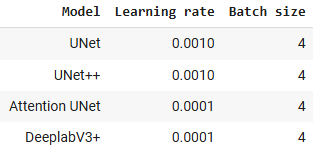
\includegraphics[scale=0.9]{IMAGENES/gridsearch.png}
%  \captionsetup{font=large}
%  \caption {Optimal hyperparameters}
% \end{figure}

\section{Preliminary training and architecture comparison}
Once the optimal hyperparameters were determined, we performed a reduced model training for each architecture using its corresponding optimal hyperparameters. As in the grid search phase, this training was performed on LoveDA Dataset only. The purpose of this stage was to determine which architecture best fits our segmentation task, and the most promising architecture identified here will later be used to perform a more complete model training, incorporating the full dataset, image augmentation, L2 regularization, etc.\\

Model evaluation was based on metrics derived from the confusion matrix. Specifically, for each architecture, predictions were generated on the validation dataset in the form of binary masks (matrices containing values of 0 and 1). These predicted masks were then compared with the corresponding ground-truth masks to construct the confusion matrix.\\

\begin{figure}[H]
 \centering
 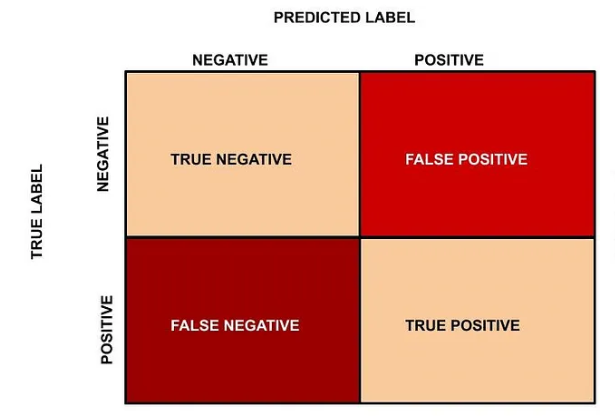
\includegraphics[scale=0.8]{IMAGENES/IMG16-CM.PNG}
 \captionsetup{font=large}
 \caption {Confusion matrix (In our case, we can consider negative as 0 and positive as 1)}
\end{figure}

The confusion matrix provides information about the number of correctly and incorrectly classified pixels, from which several metrics can be calculated to evaluate model performance. In this project, we considered three evaluation metrics:\\
\begin{itemize}
    \item \textbf{Accuracy}: This metric measures the proportion of correctly classified pixels relative to the total number of pixels, and can be determined using the following equation.\\
    \begin{equation}
    \text{Accuracy} = \frac{TP + TN}{TP + TN + FP + FN}
    \end{equation}
    \item \textbf{F1 score}: The F1 score is the harmonic mean of precision and recall, balancing false positives and false negatives, and can be determined in the following way.
    \begin{equation}
        F_{1} = \frac{2 \cdot TP}{2 \cdot TP + FP + FN}
    \end{equation}
    \item \textbf{Area under the ROC curve (AUC)}:  Since each architecture includes a final sigmoid activation layer, the raw model outputs are probability maps with values between 0 and 1 rather than strictly binary masks. To convert these into binary predictions, a threshold must be applied (for the accuracy and f1 score, we have considered a threshold of 0.5). The receiver operating characteristic (ROC) curve evaluates model performance for different threshold values, plotting the true positive rate against the false positive rate. The area under the ROC curve (AUC) summarizes this performance: a larger AUC indicates that the model is more robust and less sensitive to threshold variation. 
\end{itemize}

\section{Architecture selection}
The results obtained from the model comparison are shown in the figure below: 
\begin{table}[H]

\begin{tabular}{|c|l|l|l|l|l|}
\hline
\textbf{Architecture}            & \multicolumn{1}{c|}{\textbf{Num. of parameters}} & \multicolumn{1}{c|}{\textbf{Inference time/image (s)}} & \multicolumn{1}{c|}{\textbf{Accuracy}} & \multicolumn{1}{c|}{\textbf{F1 score}} & \multicolumn{1}{c|}{\textbf{AUC}} \\ \hline
\textbf{UNet}           & 9M                                               & 0.0047                                                 & 0.801                                  & 0.827                                  & 0.838                             \\ \hline
\textbf{UNet++}         & 31M                                              & 0.0145                                                 & 0.659                                & 0.762                                  & 0.795                             \\ \hline
\textbf{Attention UNet} & 8M                                               & 0.0063                                                 & 0.866                                  & 0.878                                  & 0.843                             \\ \hline
\textbf{DeeplabV3+}     & 41M                                              & 0.0116                                                 & 0.895                                  & 0.907                                  & 0.879                             \\ \hline
\end{tabular}
\caption{Model comparison. The table includes the number of parameters, inference time, accuracy, f1 score and AUC for each architecture.}
\label{tab:my-table}
\end{table}

%  \begin{figure}[H]
%  \centering
%  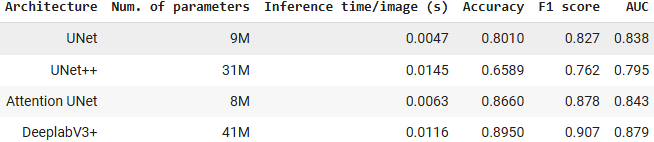
\includegraphics[scale=0.9]{IMAGENES/comparison.png}
%  \captionsetup{font=large}
%  \caption {Model comparison. The table includes the number of parameters, inference time, accuracy, f1 score and AUC for each architecture.}
% \end{figure}

As shown, DeepLabv3+ outperforms the other model architectures in all evaluation metrics, with an only drawback which is its relatively longer inference time. However, this limitation is outweighed by its high accuracy. Also, the high AUC score indicates that the architecture is robust to variations in the decision threshold. Thus, we considered that the DeepLabv3+ was the most suitable architecture for our segmentation task, and the complete training and inference in the following section were all conducted using this model architecture.\\


\section{Complete model training}
Once the best model architecture was selected, we proceeded to perform a more comprehensive training using the complete Jordan Forest and LoveDA datasets. During model training, 3 image augmentations were applied in order to enhance the model’s generalization ability. These augmentations include:\\



\begin{itemize}
    \item \textbf{Random resize crop}: A random portion of the input image is selected and resized to 512 x 512 pixels. This aims to help the model to handle images of varying resolutions. Although the training datasets contain high-resolution images, we also want to raise the model performance on lower-resolution inputs.
    \item \textbf{Color jitter}: Random modifications are applied to brightness, contrast, saturation, and hue. This helps the model adapt to variations caused by different camera setups and seasonal changes. 
    \item \textbf{Vertical and horizontal flip}: The image is randomly flipped along the horizontal or vertical axis. This augmentation may not always increase the model performance, but it is a free approach to increase training data size. 
\end{itemize}

Additionally, a L2 regularization has also been applied to prevent overfitting. This regularization introduces an additional term into the loss function that penalizes large weight values, which helps to reduce the model's complexity.

Another modification in the training process was that, instead of selecting only the best model epoch, we retained all epochs where the models achieve both an Accuracy and an F1 score greater than 0.9 on the training set (Jordan Forests and LoveDA) and greater than 0.8 on the validation set (Cantabria). We adopted a lower threshold for performance on the Cantabria set because it was not used during training, thus it would be more difficult for the model to achieve high performance on it.

The complete training resulted in 12 models, 6 were trained on the Jordan Forests Dataset and 6 on the LoveDA Dataset. We chosed to trained on these datasets separately because of the imbalance in the number of training samples and the difference in the image resolution. As mentioned earlier, the Jordan Forests Dataset contains more than 4000 images with a resolution of 2160 x 3840 pixels, whereas the Loveda Dataset has only about 300 images with a resolution of 1024 x 1024 pixels. Althogh both datasets will undergo the same preprocessing steps, which would resize all images to 512 x 512 pixels, but the imbalance in the number of samples would cause the model to be dominated and biased by the larger dataset. In order to handle this imbalance, we attempted oversampling the smaller dataset by duplicating samples and applying random augmentations. However, this has eventually led to a downgrade in model performance. Therefore, we decided to train the models separately on each dataset.\\


\chapter{Results}
In this chapter, we will present some results obtained during the project. Including inference examples and predictions performed on the tiles of the Cantabria dataset. We will also describe the post‑processing procedures applied to the model’s outputs, and finally, determine the intersection region between the vegetation and the high-voltage power lines.\\

\section{Inference examples} 
We begin by visualizing a set of inference examples. We have selected three images, each originating from one of the previously mentioned datasets. Predictions were then performed on these images using two models, one trained on the Jordan Forests Dataset and another trained on the LoveDA Dataset. 
\begin{figure}[H]
\centering
\begin{subfigure}{0.32\textwidth}
    \centering
    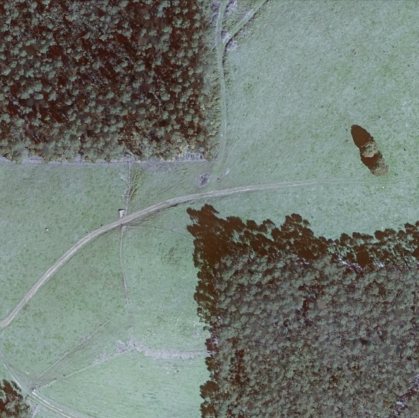
\includegraphics[width=\textwidth]{IMAGENES/Result_Img1.png}
    \caption{Cantabria Image}
    \label{fig:img1}
\end{subfigure}
\hfill
\begin{subfigure}{0.32\textwidth}
    \centering
    
\includegraphics[width=\textwidth]{IMAGENES/Result_Mask1_J.png}
    \caption{Mask (Jordan Forests Model)}
    \label{fig:img2}
\end{subfigure}
\hfill
\begin{subfigure}{0.32\textwidth}
    \centering
    
\includegraphics[width=\textwidth]{IMAGENES/Result_Mask1_Lo.png}
    \caption{Mask (LoveDA Model)}
    \label{fig:img3}
\end{subfigure}
\begin{subfigure}{0.32\textwidth}
    \centering
    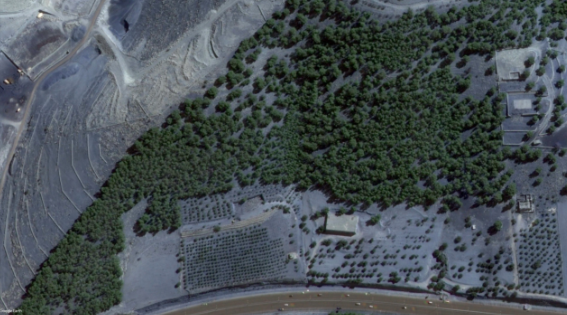
\includegraphics[width=\textwidth]{IMAGENES/Result_Img2.png}
    \caption{Jordan Forests Image}
    \label{fig:img1}
\end{subfigure}
\hfill
\begin{subfigure}{0.32\textwidth}
    \centering
    
\includegraphics[width=\textwidth]{IMAGENES/Result_Mask2_J.png}
    \caption{Mask (Jordan Forests Model)}
    \label{fig:img2}
\end{subfigure}
\hfill
\begin{subfigure}{0.32\textwidth}
    \centering
    
\includegraphics[width=\textwidth]{IMAGENES/Result_Mask2_Lo.png}
    \caption{Mask (LoveDA Model)}
    \label{fig:img3}
\end{subfigure}
\begin{subfigure}{0.32\textwidth}
    \centering
    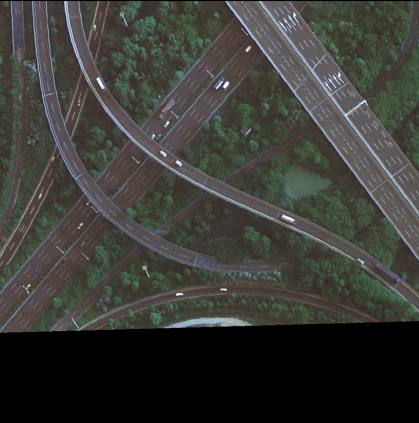
\includegraphics[width=\textwidth]{IMAGENES/Result_Img3.png}
    \caption{LoveDA Image}
    \label{fig:img1}
\end{subfigure}
\hfill
\begin{subfigure}{0.32\textwidth}
    \centering
    
\includegraphics[width=\textwidth]{IMAGENES/Result_Mask3_J.png}
    \caption{Mask (Jordan Forests Model)}
    \label{fig:img2}
\end{subfigure}
\hfill
\begin{subfigure}{0.32\textwidth}
    \centering
    
\includegraphics[width=\textwidth]{IMAGENES/Result_Mask3_Lo.png}
    \caption{Mask (LoveDA Model)}
    \label{fig:img3}
\end{subfigure}
\caption{Examples of predictions on different images using 2 models, one trained on LoveDA Dataset and another one trained on Jordan Forests Dataset.}
\label{fig:combined}
\end{figure}


As illustrated in the Figure 5.1, each model achieves good predictive results on images from its corresponding training set. However, the Jordan Forests model demonstrates poor performance on the selected LoveDA image. This limitation is because the Jordan Forests Dataset is mainly consisted of forest images, which concedes the model the ability to detect large forested areas but leaves it less effective at identifying smaller vegetation regions. In the case of the Cantabria image, both models achieved similar performance on the selected example. Nevertheless, after evaluating other images within the Cantabria dataset, we observed that the LoveDA models are more effective at capturing forest edges and smaller vegetation regions, whereas the Jordan models perform better when detecting extensive forested areas. 

\section{Inference on Cantabria dataset (Tiles)}
\subsection{Inference process}
Next, we will describe the inference process on the tiles exported during the Data Preparation stage, which differs slightly from the inference process on smaller images.


\begin{figure}[H]
 \centering
 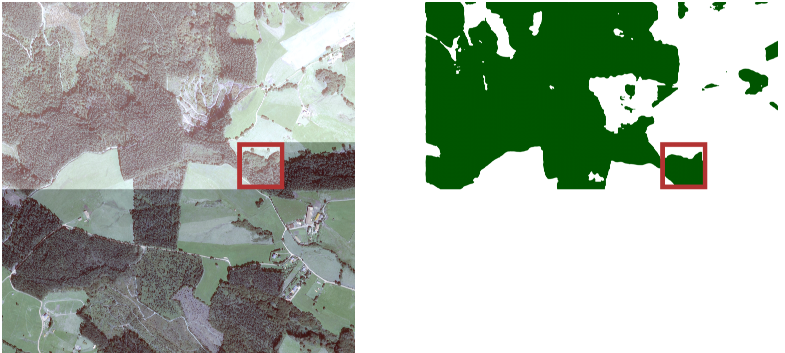
\includegraphics[scale=0.75]{IMAGENES/IMG17-Inference-process.png}
 \captionsetup{font=large}
 \caption {Inference process on Cantabria dataset. The model acts as a "sliding window" that scans over a large tile. The size of the window is 1000 x 1000 pixels.}
\end{figure}

 As previously mentioned, each tile has dimensions of 15000 x 15000 pixels, which is a very large input and therefore cannot be passed directly to the model. To perform the inference, we first loaded the entire tile into the training framework, then divided it into smaller sub-tiles of 1000 x 1000 pixels. Each sub-tile was subsequently fed into the model for prediction.  This process can be seen as using the model as a "sliding window" that scans over a large image and constructing the final mask by merging the predictions of all sub-tiles. 

\newpage


\subsection{Sharp Transitions}

The prediction mask obtained from the inference on one of the tiles is shown in the figure below: 

 \begin{figure}[H]
\centering
\begin{subfigure}{0.49\textwidth}
\centering
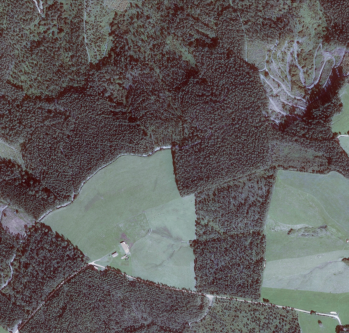
\includegraphics[width = \textwidth]{IMAGENES/IMG18-No-Aver-Img.PNG}
\caption{Cantabria dataset (Image)}
\label{fig:left}
\end{subfigure}
\begin{subfigure}{0.50\textwidth}
\centering
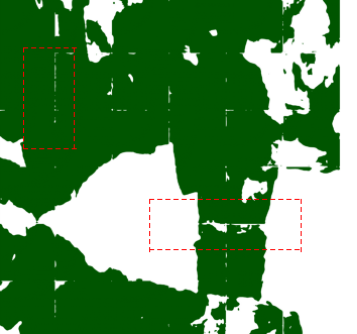
\includegraphics[width = \textwidth]{IMAGENES/IMG18-No-Aver-Mask2.PNG}
\caption{Cantabria dataset (Mask)}
\label{fig:right}
\end{subfigure}
\caption{Prediction on one of the tiles of Cantabria dataset. Dashed red rectangles highlight the regions where there are sharp transitions in the mask, these areas correspond to the junction regions between the sub-tiles.}
\label{fig:combined}
\end{figure}

As observed, there are multiple regions with sharp transition in the prediction mask, these regions align with the junction between the sub-tiles, which indicates that the model tends to perform poorly near the sub-tile boundary. One of the main reasons for this issue is that the model relies on surrounding pixels to make prediction on the target pixel. Therefore, when a forested area is divided across two sub-tiles, and one tile contains only a small fragment of the forest along its edge, it becomes difficult for the model to correctly classify these border pixels as forest. 
\newpage

\subsection{Solution}
To address this problem, one approach is to perform additional inferences on the junction regions between sub-tiles. Therefore, instead of relying on a single inference per sub-tile, 5 inferences were performed, 4 at the corners and 1 at the center.

\begin{figure}[H]
 \centering
 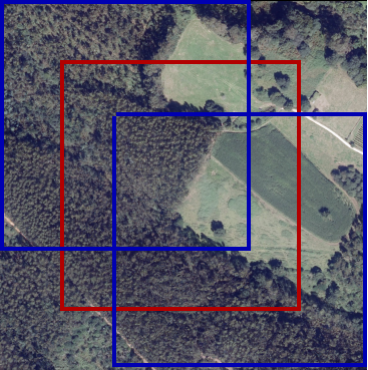
\includegraphics[scale=0.75]{IMAGENES/IMG19-Multi-inference.png}
 \captionsetup{font=large}
 \caption {Additional inferences. The red rectangle marks the target sub-tile where the prediction will be applied. For each sub-tile, 4 inferences were performed at the corners (for simplicity, this figure shows only 2 additional inferences, blue rectangles), and 1 inference was performed at the center (red rectangle).}
\end{figure}

 The corner inferences cover a subsection of the target sub-tile as well as parts from adjacent sub-tiles, providing additional contextual information to improve border pixels classification. Finally, all the inference results are averaged to produce the final output mask. The results obtained by using this approach are shown in the figure below: 
\newpage


\begin{figure}[H]
\centering
\begin{subfigure}{0.49\textwidth}
\centering

\includegraphics[width = \textwidth]{IMAGENES/IMG20-Aver-Mask.png}
\caption{Prediction mask with additional inferences.}
\label{fig:left}
\end{subfigure}
\begin{subfigure}{0.49\textwidth}
\centering

\includegraphics[width = \textwidth]{IMAGENES/IMG18-No-Aver-Mask.png}
\caption{Prediction mask without additional inferences.}
\label{fig:right}
\end{subfigure}
\caption{Comparison between the prediction with and without averaging.}
\label{fig:combined}
\end{figure}

As shown, there is a significant improvement in the prediction mask, particularly along the borders of the sub-tiles where sharp transitions were previously visible. Additionally, since the final mask is obtained by averaging the results from multiple inferences, there is also an increase in the prediction accuracy.\\


\section{Postprocessing}

In order to determine the intersection areas between the vegetation and power lines, the masks obtained from the previous section must be further processed. This postprocessing step included adding georeferencing information and converting the masks into a more suitable format to simplify the calculation of intersection areas.\\

The georeferencing was performed by using a Python script with the GDAL library, which merged each mask with its corresponding georeferencing file and converted it from PNG to GeoTIFF (a georeferenced raster image). Regarding the mask conversion, one option considered during the project was to transform the raster masks into tables of coordinates. In other words, each vegetation pixel would be converted into its corresponding latitude and longitude values and stored as a vector. These vegetation coordinates could then be loaded alongside the power line data, and the intersections were determined by using functions from GeoPandas library.\\

However, storing pixel level coordinates presented a significant drawback, which is that the computation time for intersection detection was extremely long due to the large number of pixels involved, because the algorithm needed to scan every pixel and evaluate whether it intersected with the power line data. Therefore, to accelerate processing time, an alternative approach was adopted: Instead of converting all vegetation pixels into coordinates, only the contour coordinates of each vegetation object in the prediction mask were extracted and stored.\\

 \begin{figure}[H]
\centering
\begin{subfigure}{0.49\textwidth}
\centering
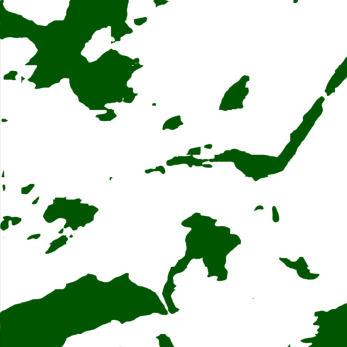
\includegraphics[width = \textwidth]{IMAGENES/IMG21-Contour1.png}
\caption{Prediction mask.}
\label{fig:left}
\end{subfigure}
\begin{subfigure}{0.49\textwidth}
\centering

\includegraphics[width = \textwidth]{IMAGENES/IMG21-Contour2.png}
\caption{Contours of vegetation objects.}
\label{fig:right}
\end{subfigure}
\begin{subfigure}{0.60\textwidth}
\centering
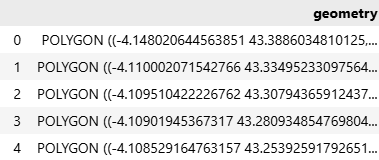
\includegraphics[width = \textwidth]{IMAGENES/IMG21-Contour3.png}
\caption{Contours stored as geometry objects.}
\label{fig:right}
\end{subfigure}
\caption{(a)->(b)->(c) shows the process of converting prediction mask into coordinates.}
\label{fig:combined}
\end{figure}

The contours extraction was achieved by using a function from the OpenCV library, which detects contours of each object in binary images based on the algorithm proposed in this paper [26]. Once extracted, the contour coordinates were converted into geometry objects (commonly used format for handling geospatial data) using the Shapely library. These objects are represented as text strings (Figure 5.6.c) that contain coordinate information, preceded by a header that specifies the geometry type (for vegetation objects, the extracted contours were stored specifically as polygons), and the GeoPandas library can directly parse and interpret this format. 


\section{Intersection with power line}
After converting the prediction masks into coordinates and saving them as geometry objects, these were combined with the power line data to determine the intersection areas. To ensure compatibility, the power line dataset was also converted into geometry objects, stored specifically as StringLines. \\

Since the aim of the projects was to identify potential contact regions rather than exact contact points, a buffering step was applied to the power line geometries. This buffer expanded the lines by a given margin, creating a zone that represents the potential contact area (see figure below). And every vegetation polygon falling inside this buffered zone was flagged as a risk zone. 

\begin{figure}[H]
 \centering
 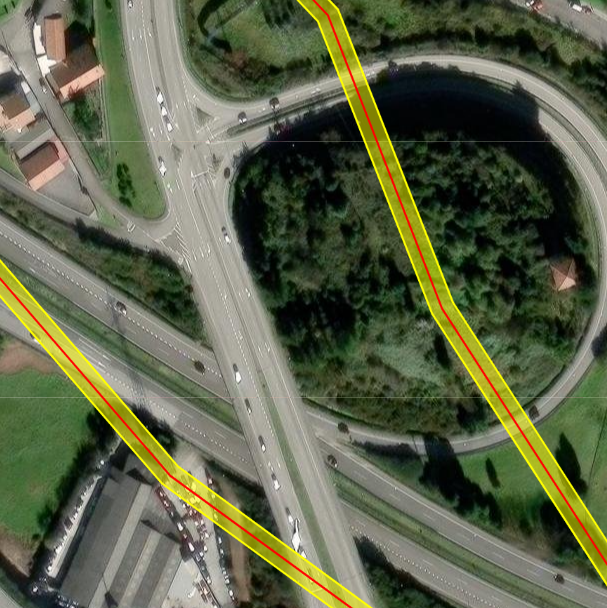
\includegraphics[scale=0.49]{IMAGENES/IMG22-PowerLine2.png}
 \captionsetup{font=large}
 \caption {Power line data. The red lines represent the power line coordinates, and the yellow zones correspond to the buffer.}
\end{figure}

Some examples of the intersection areas are shown in the figure below: 

 \begin{figure}[H]
\centering
\begin{subfigure}{0.32\textwidth}
\centering
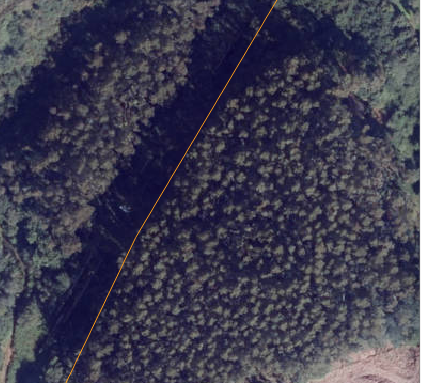
\includegraphics[width = \textwidth]{IMAGENES/Intersection1.png}
\caption{Raster image.}
\label{fig:left}
\end{subfigure}
\begin{subfigure}{0.328\textwidth}
\centering
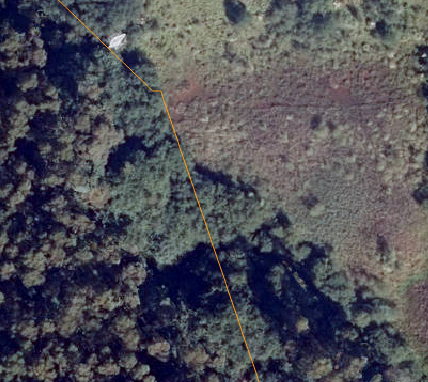
\includegraphics[width = \textwidth]{IMAGENES/Intersection2.png}
\caption{Raster image.}
\label{fig:right}
\end{subfigure}
\begin{subfigure}{0.305\textwidth}
\centering
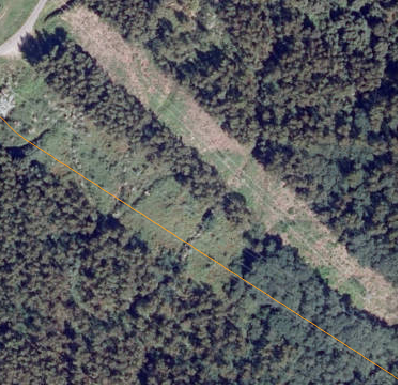
\includegraphics[width = \textwidth]{IMAGENES/Intersection3.png}
\caption{Raster image.}
\label{fig:left}
\end{subfigure}
\begin{subfigure}{0.31\textwidth}
\centering
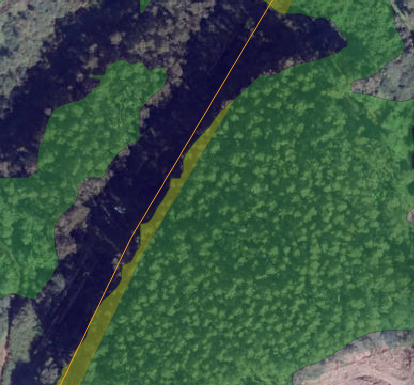
\includegraphics[width = \textwidth]{IMAGENES/Intersection1-m.png}
\caption{Intersection areas for figure (a).}
\label{fig:right}
\end{subfigure}
\begin{subfigure}{0.33\textwidth}
\centering
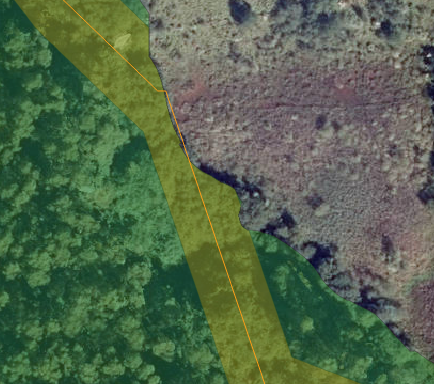
\includegraphics[width = \textwidth]{IMAGENES/Intersection2-m.png}
\caption{Intersection areas for figure (b).}
\label{fig:right}
\end{subfigure}
\begin{subfigure}{0.31\textwidth}
\centering
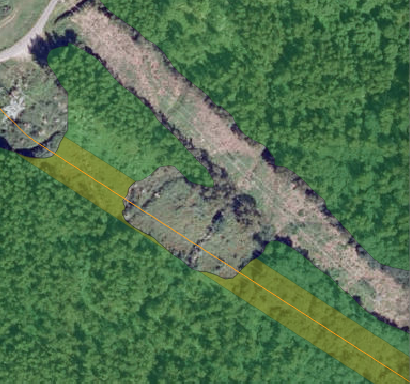
\includegraphics[width = \textwidth]{IMAGENES/Intersection3-m.png}
\caption{Intersection areas for figure (c).}
\label{fig:left}
\end{subfigure}
\caption{Examples of intersection areas. }
\label{fig:combined}
\end{figure}

As illustrated, several risk zones were detected where potential contact between power lines and vegetation could occur. In certain regions, the power lines do not actually come into contact with the trees (Figures 5.8.a and 5.8.b), because the utility poles are significantly taller than the surrounding vegetation. However, there are also some other risk zones that appear as a result of misclassified forest pixels (Figure 5.8.c). After evaluating other intersection areas, we have concluded that this degradation in the model performance could be attributed mainly to 2 factors: 

\begin{itemize}
    \item \textbf{Differences in vegetation species}: The models were trained on forest imagery from Jordan and China, but predictions were performed on forests in Cantabria. Thus, the variation in vegetation types across regions could produce distinct textural patterns in satellite imagery. Since the training data may not have included sufficient examples of forest types, the models were less effective in generalizing to Cantabria images, leading to misclassifications. 
    \item \textbf{Image resizing}: As previously mentioned, the input images have been resized to 512 x 512 pixels regardless of their original dimensions in order to reduce memory consumption. However, this resizing process has also led to the loss of fine details due to compression. This is a major drawback because these details are often relevant for pixel-level classification, and working with smaller images increases the difficulty for the model to correctly capture the shape and boundaries of tree canopies.  
\end{itemize}

In conclusion, while the models have identified the majority of vegetation areas, some detected regions present false positives due to certain limitations. Specifically, these limitations stem from insufficient variability in the training data and from transformations applied to the training images as a consequence of the high computational requirements. Although some of these limitations might be unavoidable, several improvements have been considered for a potential future work to improve the accuracy of the vegetation identification and intersection analysis. \\

\section{Future directions}
\begin{itemize}
    \item \textbf{High quality labeled Cantabria dataset}: The most direct way to increase the model performance on Cantabria images is to train the model on the forest images of Cantabria (or similar forested regions in Spain). However, as mentioned before, this is usually a time-consuming task as it requires manual annotation of forested areas.  
    \item \textbf{Pretrained backbone}: The DeeplabV3 models in this project employ a backbone pretrained on the ImageNet-1k dataset, which contains images that are not directly relevant to forest segmentation task. A more suitable strategy would be to use a backbone pretrained on Cantabria forest images, which would allow the model to become “familiar” with the forest species in this region. Furthermore, since the backbone primarily serves as a feature extractor, it can be pretrained using self-supervised learning methods that do not require labeled data. 
    \item \textbf{Exploration of alternative architectures}: In this project, only four architectures were tested. These models can be served as useful benchmarks for comparing other architectures that may achieve superior performance on vegetation segmentation tasks. For instance, transformer-based architectures (SegFormer or Mask2Former) have shown strong performance in recent computer vision research. Additionally, some lightweight architectures optimized for remote sensing could offer a better balance between accuracy and computational efficiency. 
\end{itemize}

 



 




 

 

 






 









\chapter{Gradio Application}
To demonstrate the model's capabilities and visualize the results interactively, we have developed a web application that integrates some of the previously mentioned features into a user-friendly interface using the Gradio framework. The application is designed with two main modules: the first for image segmentation, and the second for an AI assistant chatbot that helps users interact with vegetation and high-voltage network coordinates.
\section{Image Segmentation Module}
\begin{figure}[H]
 \centering
 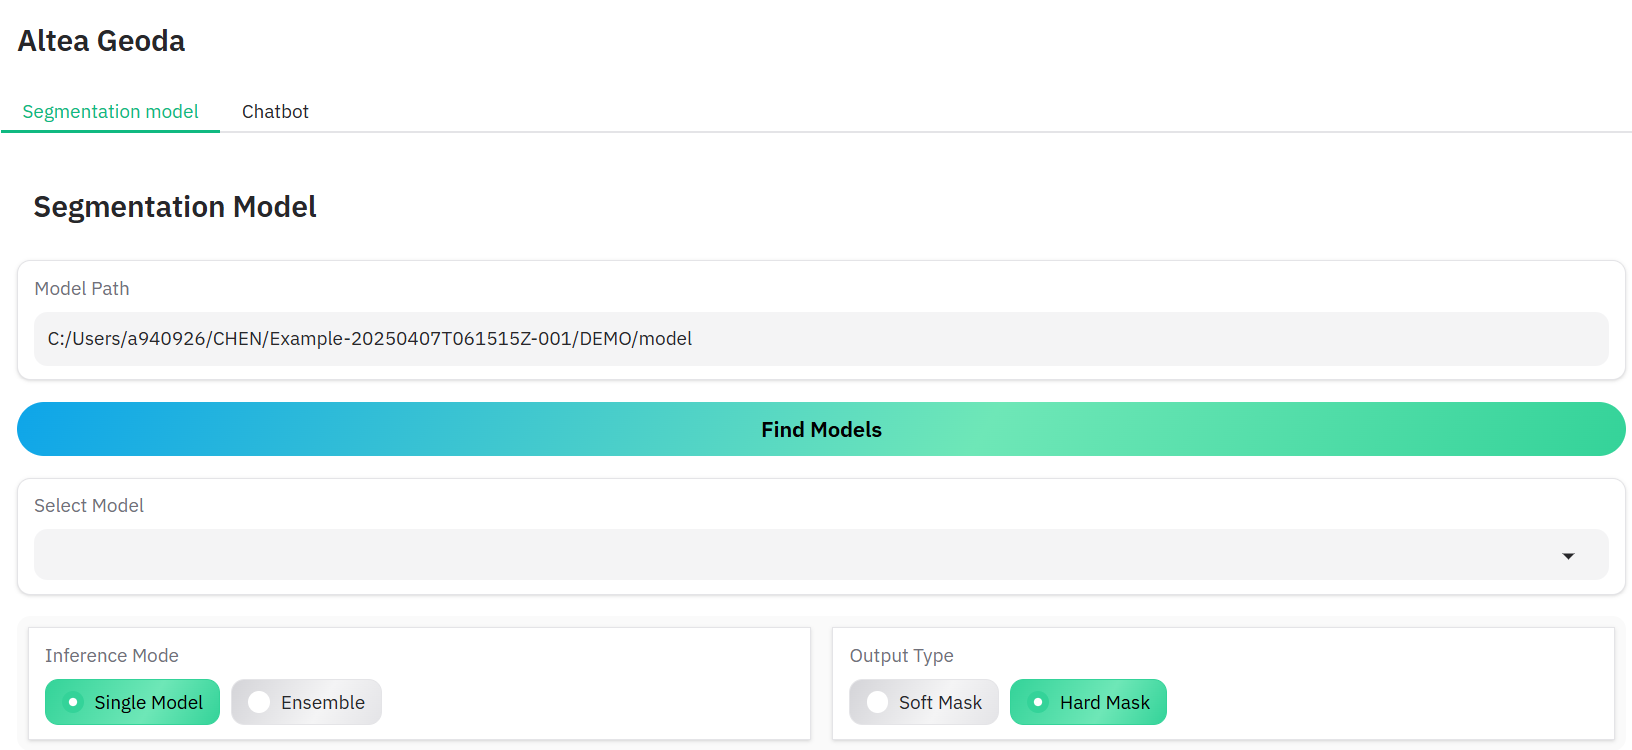
\includegraphics[scale=0.55]{IMAGENES/Gradio_app_segmentation1.png}
 \captionsetup{font=large}
 \caption {Gradio application (Image segmentation module).}
\end{figure}
In this module, users can upload a custom image and visualize the segmentation results directly in the browser. To perform inference, the user needs to specify the path to the directory where the model weights are stored. The pre-trained weights can be downloaded from the provided link [26], which contains six pre-trained models. Each model is named according to the dataset it was trained on, along with its corresponding training and testing accuracy. Users can either select a specific model for prediction or use an ensemble of all models for more robust results. Additionally, the application offers an option to choose the output type: Soft mask (outputs the raw probability map generated by the model) or Hard mask (Outputs a binary mask obtained by thresholding the soft mask at 0.5). There are no strict restrictions on the input image size or format, as the application automatically resizes the image to 512 x 512 pixels, which is the required input size for the model. However, for optimal performance, we recommend using images with dimensions close to 1024 x 1024 to 2048 x 2048 pixels, as these sizes match the training data.
\begin{figure}[H]
 \centering
 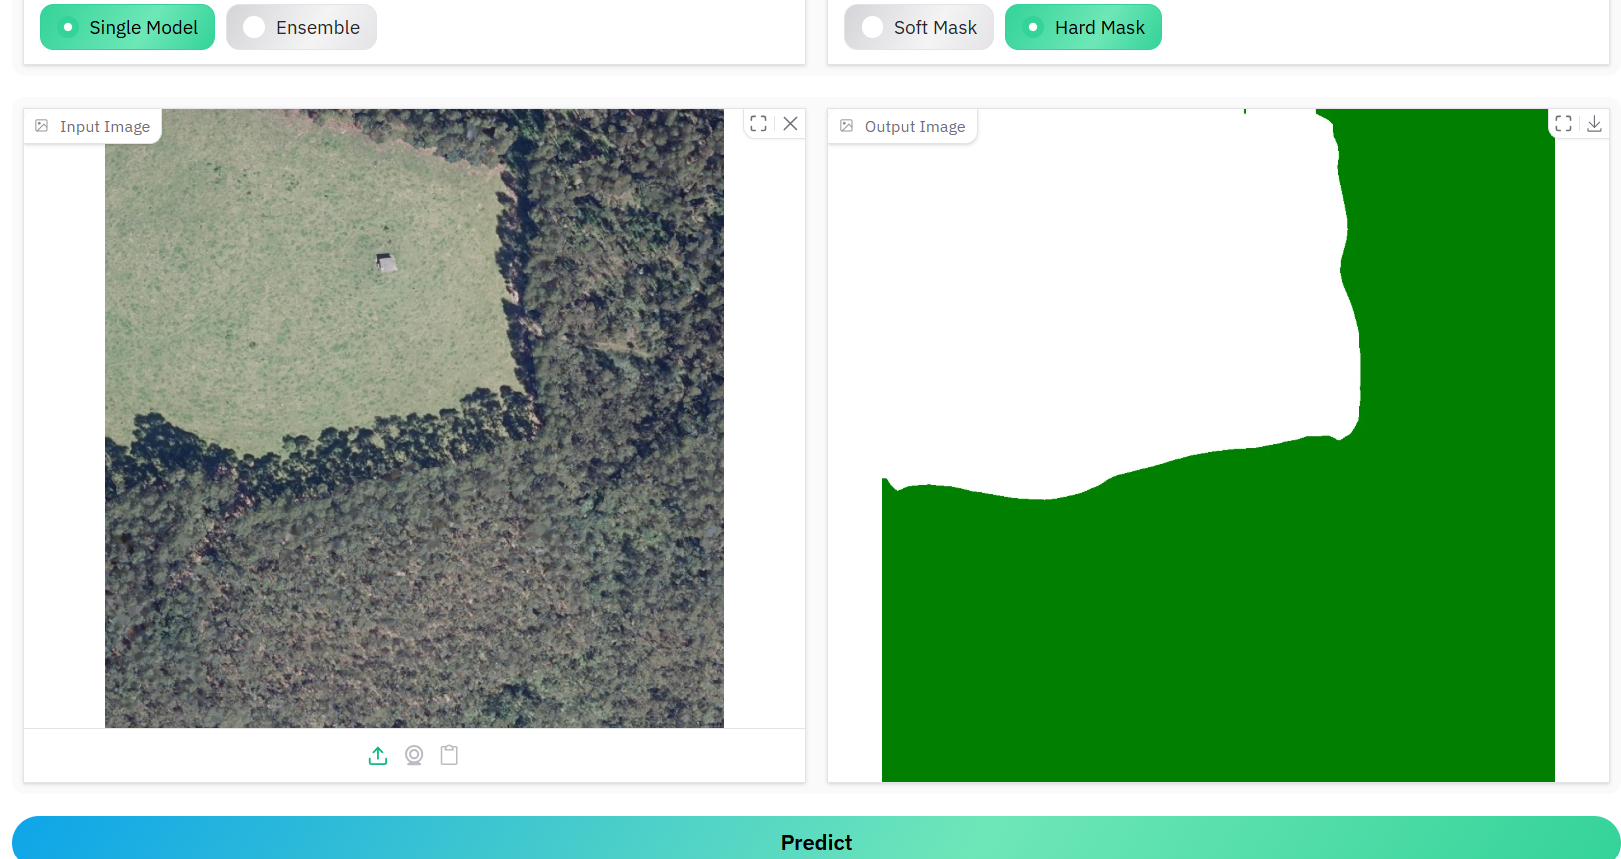
\includegraphics[scale=0.55]{IMAGENES/Gradio_app_segmentation2.png}
 \captionsetup{font=large}
 \caption {Gradio application (Image segmentation module).}
\end{figure}

\section{Ai Agent Assistant}
The second module is a chatbot assistant to interact with the coordinates of vegetation and high-voltage network. We provided all of our prediction results as coordinates stored in a CSV file, which contains 70 tiles in the Cantabria region, with each tile assigned a unique ID. Users can perform various queries through the chatbot to generate vegetation distribution, intersection or risk zone graphs. These queries can be made using either the tile ID, a specific location name or address.

\subsection{How the Chatbot Works}
The chatbot is built using an agent framework (LangGraph). An AI agent in this context refers to a language-model-powered system that can interact with external tools or environments and perform actions autonomously to achieve different objectives. In this application, we implemented a single agent with access to three primary tools:
\begin{itemize}
    \item \textbf{Display graph tool}: Displays graphs for a specific region based on the ID provided by the user.
    \item \textbf{Geocode tool}: Retrieves geographical coordinates based on a location name or address.
    \item \textbf{Get-id tool}: Finds the tile ID corresponding to a set of coordinates.
\end{itemize}
\textbf{Example Query}:\\
If the user asks:
"Display the intersection graph for Maliaño"
\begin{figure}[H]
 \centering
 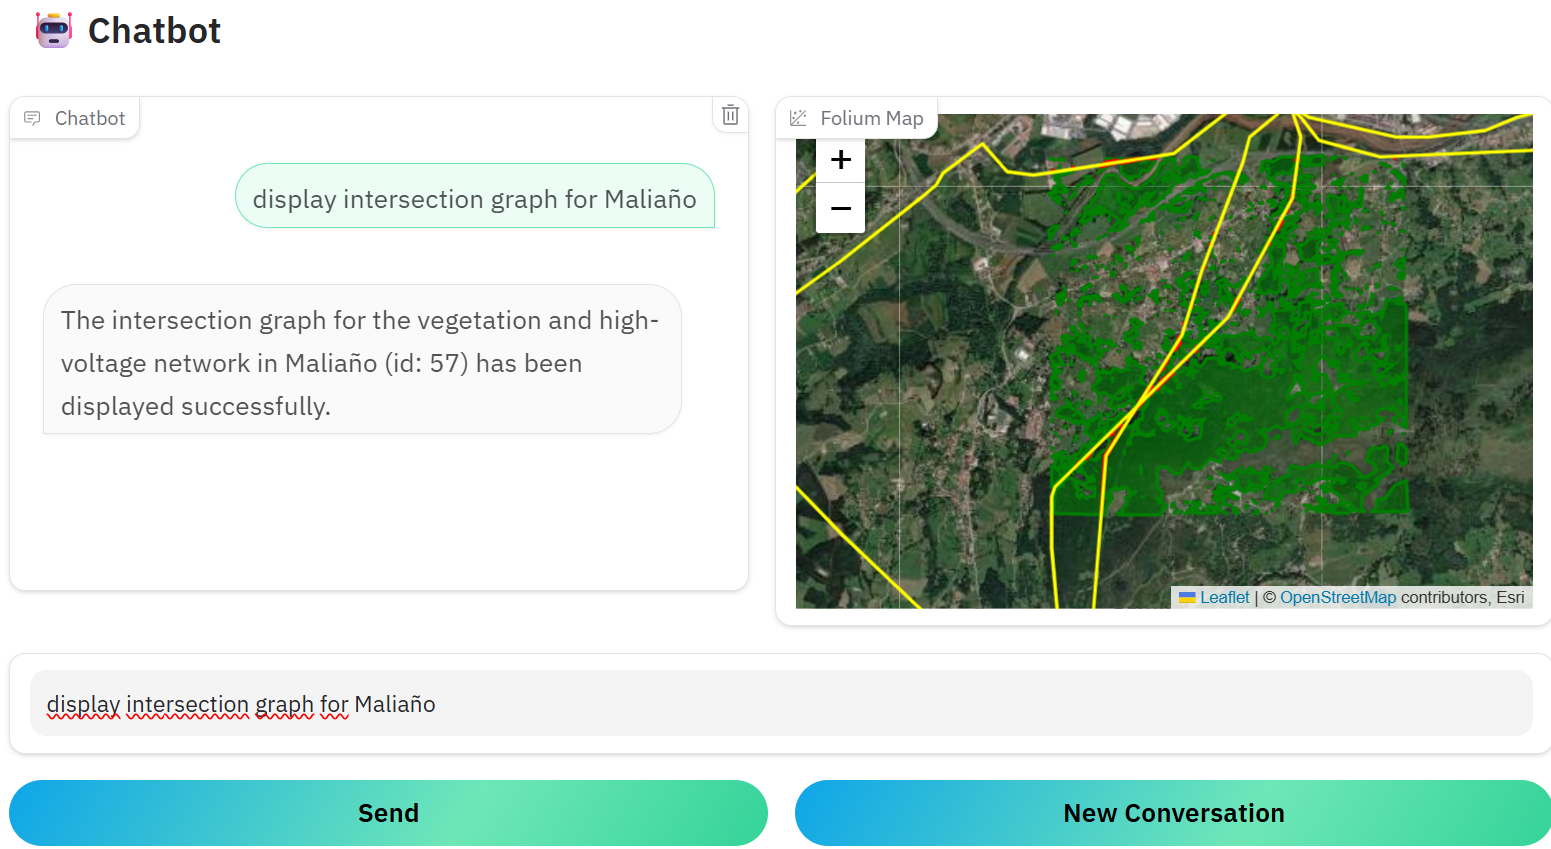
\includegraphics[scale=0.55]{IMAGENES/Gradio_app_chatbot.png}
 \captionsetup{font=large}
 \caption {Gradio Application (AI Agent Module): The module consists of two components. On the left, the user can view the chat history with the agent, and on the right, the user can view the queried graph on an interactive map.}
\end{figure}



the agent will follow these steps:
\begin{itemize}
    \item Call \textbf{Geocode tool} to retrieve the coordinates of "Maliaño".
    \item Call \textbf{Get-id tool} to determine the tile ID associated with those coordinates.
    \item Call \textbf{Display graph tool} to generate and display the vegetation distribution graph for the corresponding tile.
\end{itemize}
Beyond the basic query functionality, the chatbot supports advanced options, such as: Modifying the buffer size around high-voltage lines when generating intersection graphs. Or retrieving the addresses of the risk zone with largest area:

\begin{figure}[H]
 \centering
 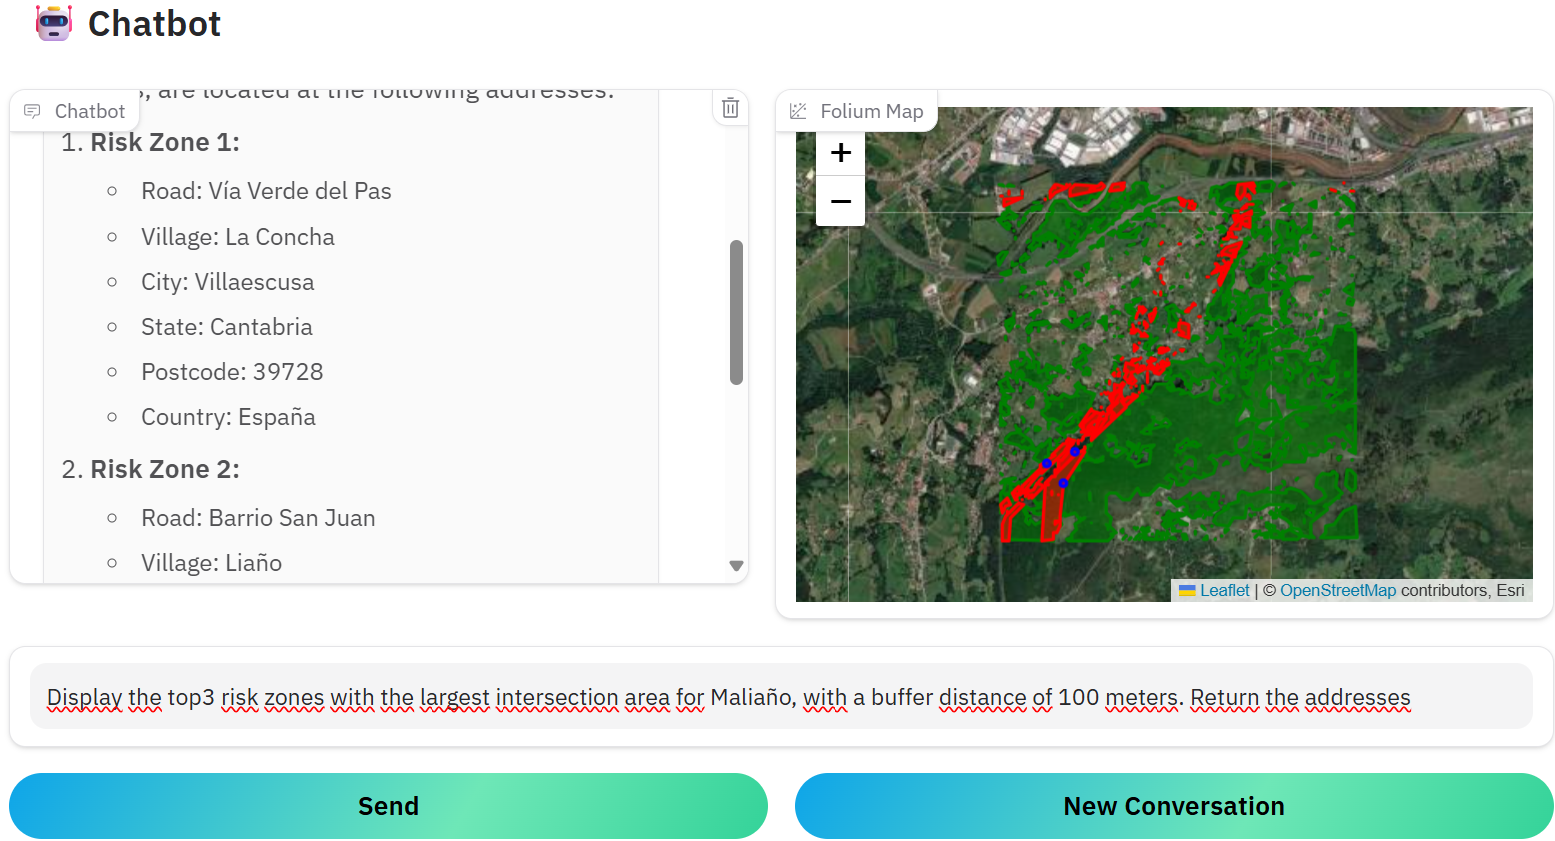
\includegraphics[scale=0.37]{IMAGENES/Gradio_app_chatbot2.png}
 \captionsetup{font=large}
 \caption {Gradio Application (AI Agent Module)}
\end{figure}

In this example, the buffer size is set to 100 meters, illustrating that the agent allows dynamic adjustment of this parameter. Additionally, the addresses of the top 3 zones with the largest intersection areas are displayed in the chat history.\\







\chapter{Conclusion}
In this project, four architectures were evaluated for the forest segmentation task, with DeepLabV3+ achieving the best overall performance across Accuracy, F1-score, and AUC. Using this architecture, 12 models were trained on two different datasets: 6 on the Jordan Forest dataset and 6 on the LoveDA dataset. When evaluated on Cantabria forest images, the LoveDA-trained models demonstrated greater effectiveness in capturing fine details such as edges and small vegetation, while the Jordan-trained models proved more reliable in detecting larger forested areas.\\

The models were then applied to a larger region of Cantabria, divided into 70 tiles of 3000m x 3000m each. The resulting prediction masks were transformed into geospatial coordinates and integrated with power line data to identify potential intersection zones. During this process, some false-positive contact regions were observed, likely caused by the limited variety of training samples and the preprocessing step of resizing all input images to 512 × 512 pixels.\\

Finally, a web application was developed to integrate these functionalities, offering an interactive interface for custom image segmentation and a chatbot assistant to facilitate exploration of the results. The full code implementation is publicly available in the GitHub repository [27]. Note: The chatbot module relies on the Azure OpenAI API, meaning that an active OpenAI API endpoint must be provided in the code to enable this functionality.








%:Para incluir toda la referencia bibliográfica aunque no se cite, descomente la siguiente línea
\nocite{*}

%:Empieza todo lo que no constituye el cuerpo en si del libro. Todo lo que va detrás
\backmatter





%BIBTEX
%%\bibliographystyle{IEEEtran}
%\bibliographystyle{amsplain} %flexbib amsplain alpha
%%:Fichero con la bibliografía, BIBTEX
%\bibliography{bibliografiatermo}
%\renewcommand{\bibname}{Bibliografía}
%cuerpo posterior del book
%\addcontentsline{toc}{chapter}{Bibliografía}
\bibliographystyle{ieeetr}
\bibliography{biblioTFG}

%:Índice alfabético
%\only<article>{
%\cleardoublepage
%\phantomsection
%\addcontentsline{toc}{listasb}{\indexname}
% \sectionmark{\indexname}
%\printindex
%}

\cleardoublepage

%:Empezamos con los apéndices, que irían en uno o más ficheros. Es necesario incluir estos ficheros entre el entorno \begin{appendices}....\end{appendices} debido a que se ha deseado utilizar un formato diferente para el título de los apéndices, incluyendo la palabra apéndice, para la numeración de los apéndices, alfabético, y para las cabeceras de las páginas.
%\begin{appendices}
% Fichero en el que se incluyen los apéndices
%\include{apendices/apendices} %Ver este fichero para incluir ahí los apéndices.
%\end{appendices}
%:Fin de la inclusión de apéndices

\appendix
%% Activate the following line by filling in the right side. If for example the name of the root file is Main.tex, write
% "...root = Main.tex" if the chapter file is in the same directory, and "...root = ../Main.tex" if the chapter is in a subdirectory.
 
%!TEX root =  ../plantillaTFG.tex 
%recuerda que si cambias el nombre del fichero... debes cambiarlo aqui
\chapter{Anexo}

\cite{apd}
\cleardoublepage
\include{./CAPITULOS/codigo}
\cleardoublepage

\listoffigures

\listoftables


\end{document}
